\documentclass[12pt,t]{beamer}
\usepackage[utf8]{inputenc}
\usepackage[catalan]{babel}
\usepackage{verbatim}
\usepackage{hyperref}
\usepackage{amsfonts,amssymb,amsmath,amsthm, wasysym}
\usepackage{listings}
\usepackage[T1]{fontenc}        
\usepackage{pgf}
\usepackage{epsdice}
\usepackage{pgfpages}
\usepackage{tikz}
\setbeamertemplate{caption}[numbered]
\setbeamertemplate{navigation symbols}{}


\newcommand{\red}[1]{\textcolor{red}{#1}}
\newcommand{\green}[1]{\textcolor{green}{#1}}
\newcommand{\blue}[1]{\textcolor{blue}{#1}}
\newcommand{\gray}[1]{\textcolor{gray}{#1}}
\renewcommand{\emph}[1]{{\color{red}#1}}

\setbeamertemplate{frametitle}
{\begin{centering}
\smallskip
\color{blue}
\textbf{\insertframetitle}
\end{centering}
}
\usecolortheme{rose}
\usecolortheme{dolphin}
\mode<presentation>


\newcommand{\CC}{\mathbb{C}}
\newcommand{\RR}{\mathbb{R}}
\newcommand{\ZZ}{\mathbb{Z}}
\newcommand{\NN}{\mathbb{N}}
\newcommand{\KK}{\mathbb{K}}
\newcommand{\MM}{\mathcal{M}}
%\newcommand{\dbinom}{\displaystyle\binom}

\newcommand{\limn}{{\displaystyle \lim_{n\to\infty}}}
\renewcommand{\leq}{\leqslant}
\renewcommand{\geq}{\geqslant}
\def\tendeix{{\displaystyle\mathop{\longrightarrow}_{\scriptscriptstyle
n\to\infty}}}

\newcommand{\matriu}[1]{\left(\begin{matrix} #1 \end{matrix}\right)}

% \newcommand{\qed}{\hbox{}\nobreak\hfill\vrule width 1.4mm height 1.4mm depth 0mm
%     \par \goodbreak \smallskip}
%
% %
\theoremstyle{plain}
\newtheorem{teorema}{Teorema}
\newtheorem{prop}{Proposició}
\newtheorem{cor}{Coro\l.lari}
\theoremstyle{definition}
\newtheorem{exemple}{Exemple}
\newtheorem{defin}{Definició}
\newtheorem{obs}{Observació}

\newcounter{seccions}
\newcommand{\seccio}[1]{\addtocounter{seccions}{1}
\medskip\par\noindent\emph{\theseccions.
#1}\smallskip\par }

\newcommand{\EM}{\Omega}
\newcommand{\PP}{\mathcal{P}}

\usepackage{listings}

\lstset{
language=R, %
aboveskip=1 ex, %
belowskip=-4ex, %
linewidth=\textwidth,
%xleftmargin=0.5cm,
%xrightmargin=0.5cm,
basicstyle={\footnotesize\ttfamily}, %
commentstyle=\ttfamily\color{red}, %
numbers=none, %
%morecomment=[l]{E},
numberstyle=\ttfamily\color{gray}\footnotesize,
stepnumber=1,
numbersep=5pt,
backgroundcolor=\color{gray!15},%15
showspaces=false,
%showstringspaces=false,
showtabs=false,
frame=single, %????
framerule=0pt,
keepspaces=true,
tabsize=2,
captionpos=b, %
breaklines=true, %
breakatwhitespace=false,  %
showstringspaces=false,
title=\lstname,
literate={{á}{{\'a}}1 {é}{{\'e}}1 {í}{{\'i}}1 {ó}{{\'o}}1 {ú}{{\'u}}1
  {Á}{{\'A}}1 {É}{{\'E}}1 {Í}{{\'I}}1 {Ó}{{\'O}}1 {Ú}{{\'U}}1
  {à}{{\`a}}1 {è}{{\`e}}1 {ì}{{\`i}}1 {ò}{{\`o}}1 {ù}{{\`u}}1
  {À}{{\`A}}1 {È}{{\'E}}1 {Ì}{{\`I}}1 {Ò}{{\`O}}1 {Ù}{{\`U}}1
  {ä}{{\"a}}1 {ë}{{\"e}}1 {ï}{{\"i}}1 {ö}{{\"o}}1 {ü}{{\"u}}1
  {Ä}{{\"A}}1 {Ë}{{\"E}}1 {Ï}{{\"I}}1 {Ö}{{\"O}}1 {Ü}{{\"U}}1 {ñ}{{\~n}}1 {Ñ}{{\~N}}1
  {â}{{\^a}}1 {ê}{{\^e}}1 {î}{{\^i}}1 {ô}{{\^o}}1 {û}{{\^u}}1
  {Â}{{\^A}}1 {Ê}{{\^E}}1 {Î}{{\^I}}1 {Ô}{{\^O}}1 {Û}{{\^U}}1
  {œ}{{\oe}}1 {Œ}{{\OE}}1 {æ}{{\ae}}1 {Æ}{{\AE}}1 {ß}{{\ss}}1
  {ç}{{\c c}}1 {Ç}{{\c C}}1 {ø}{{\o}}1 {å}{{\r a}}1 {Å}{{\r A}}1
  {€}{{\EUR}}1 {£}{{\pounds}}1 {¡}{{\textexclamdown}}1 {¿}{{\textquestiondown}}1 {!}{{!}}1
  {·}{{\textperiodcentered}}1}
 }
 
\lstdefinestyle{warning}{basicstyle={\footnotesize\ttfamily\color{red}}}



\title[\red{Matemàtiques II}]{}
\author[]{}
\date{}



\begin{document}
\beamertemplatedotitem

\begin{frame}
\vfill
\begin{center}
\gray{\LARGE\bf ANOVA d'1 via}
\end{center}
\end{frame}

\begin{frame}
\frametitle{Exemple}
\blue{Es jutja amb més benevolència a una persona segons com somriu?}\medskip

136 persones, dividides a l'atzar en 4 grups de 34.\medskip

A les persones de cada grup se'ls passà un dossier on s'acusava a un home d'una falta greu i sel's demanà 5 preguntes sobre la culpabilitat de l'interfecte i el càstig.\medskip

A partir de les  respostes de  cada subjecte, es calculà un \emph{índex de benevolència}  de com havia jutjat l'acusat.\medskip

Els dossiers eren idèntics, excepte la foto de l'acusat: mateix home, però diferent tipus de somriure.

\end{frame}

\begin{frame}
\frametitle{Exemple}


\begin{center}
\hspace*{-0.5cm}\begin{tabular}{cccc}

\includegraphics[width=0.24\linewidth]{felt} & 

\includegraphics[width=0.26\linewidth]{false} & 

\includegraphics[width=0.22\linewidth]{miserable} & 

\includegraphics[width=0.25\linewidth]{neutral}\\
Sincer & Fals & Compungit & Neutre
\end{tabular}
\end{center}\pause

Dades a \blue{\url{https://raw.githubusercontent.com/AprendeR-UIB/MatesIIAD/master/dades/smiles.txt}}\vspace*{1cm}

{\tiny M. LaFrance, M. Hecht, \textsl{Personality and Social Psychology Bulletin} 21 (1995) 207--214

}
\end{frame}

\begin{frame}
\frametitle{Exemple}

Resultats: 
\begin{center}
\begin{tabular}{cccc}
\multicolumn{4}{c}{Tipus de somriure}\\\hline
Sincer & Fals & Compungit & Neutre\\\hline
6.5 &4.5 &  5.0  &  4.0 \\
4.5 &3.5 & 6.5  &  2.5  \\
4.0 &7.5 & 6.0  &  2.5  \\
7.0  &6.5 & 5.0  &  2.5  \\
5.5 & 3.0 & 5.5  & 2.0  \\
5.0  &3.0 & 3.5  &  5.0  \\
4.5  &5.5 & 4.0  & 2.5  \\
6.0 & 6.0 &5.5  &6.0    \\
$\vdots$ & $\vdots$ & $\vdots$ & $\vdots$ 
\end{tabular}
\end{center}\pause\medskip

\blue{L'índex mitjà de benevolència, depèn del tipus de somriure de la foto?}
\end{frame}



\begin{frame}
\frametitle{Exemple}

\red{Variables d'interès}\medskip
\begin{itemize}
\item $X$: Índex de benevolència d'una persona a qui s'ha mostrat una foto de l'acusat\smallskip

\item $X_s$: Índex de benevolència d'una persona a qui s'ha mostrat una foto amb un somriure sincer de l'acusat\medskip

\item $X_f$, $X_c$, $X_n$: Ídem, amb somriure fals, compungit i neutre
\end{itemize}
\medskip

Siguin $\mu_s,\mu_f,\mu_c,\mu_n$ les seves mitjanes\medskip

\red{Contrast}
$$
\left\{
\begin{array}{l}
H_0 : \mu_s=\mu_{f}=\mu_{c}=\mu_{n} \\
H_1 : \mbox{Hi ha  somriures }i,j\mbox{ tals que }  \mu_i \not=\mu_j
\end{array}
\right.
$$

\end{frame}



\begin{frame}
\frametitle{Situació general}

\begin{itemize}
\item Hem emprat un únic factor per classificar la població en 4 subpoblacions (el tipus de somriure)\medskip




\item Hem pres una m.a.s.  cada subpoblació,  independents les unes de les altres
\end{itemize}\pause\medskip


\begin{itemize}
\item \red{$\mu$}: mitjana poblacional  del conjunt de la població  (ignorant els nivells)
\medskip

\item \red{$\mu_i$}: mitjana poblacional dins el nivell $i$-èsim,
$i=1,\ldots,k$
\medskip
\end{itemize}\medskip

\red{Contrast}:
$$
\left\{
\begin{array}{l}
H_0 : \mu_1=\mu_{2}=\cdots=\mu_{k} \\
H_1 : \mbox{Hi ha  }i,j\mbox{ tals que }  \mu_i \not=\mu_j
\end{array}
\right.
$$\pause\medskip

Si $H_0: \mu_1=\cdots=\mu_k$ és certa, aleshores
$$
\mu_1=\cdots=\mu_k=\mu
$$

\end{frame}




\begin{frame}
\frametitle{Problema general}

$$
\left\{
\begin{array}{l}
H_0 : \mu_1 =\mu_2 =\cdots =\mu_k \\
H_1 : \mbox{Hi ha  }i,j\mbox{ tals que }  \mu_i \not=\mu_j
\end{array}
\right.
$$\

$H_1$ \red{no és}
\begin{center}
\blue{totes les mitjanes són diferents}
\end{center}
sinó
\begin{center}
\blue{hi ha almenys dues mitjanes que són diferents}
\end{center}
\end{frame}



\begin{frame}
\frametitle{Problema general}

\red{En capítols anteriors:} Per comparar les mitjanes de dues vv.aa.,  calculàvem les mitjanes de dues mostres i les comparàvem
\medskip

Per comparar les mitjanes de $k\geq 3$ vv.aa., podríem fer-ho per parelles, però hauríem de fer $\binom{k}{2}$ contrastos i augmenta la probabilitat d'error
\medskip

I les hem de comparar totes amb totes, perquè pot passar que
\begin{itemize}
\item No poguem rebutjar que $\mu_1= \mu_2$
\item No poguem rebutjar que $\mu_2= \mu_3$
\item \textit{Sí} que poguem rebutjar que $\mu_1= \mu_3$
\end{itemize}
\medskip

Volem un test que ens digui en un pas si totes són iguals, o si n'hi ha de diferents (en aquest darrer cas, ja cercarem les diferents si volem)
\end{frame}


\begin{frame}
\frametitle{ANOVA}

La tècnica més usual és l'\emph{Anàlisi de la Variància} (\emph{ANOVA}, de l'anglès \textsl{\red{AN}alysis \red{O}f \red{VA}riance})
\bigskip

Aquesta tècnica es pot aplicar sota diferents dissenys experimentals:\medskip

\begin{itemize}
\item Segons quants factors empram per separar la població en subpoblacions
\medskip

\item Segons com triam els nivells dels factors
\medskip

\item Segons com prenem les mostres
\end{itemize}
\medskip

El que estam fent és \emph{ANOVA d'1 via}: 1 sol factor, mostres independents.


\end{frame}




\begin{frame}
\frametitle{ANO\ldots VA?}

Per comparar les mitjanes de 3 o més poblacions, ens fixam en les fonts de variabilitat de les dades:
\medskip

\begin{itemize}
\item \blue{Variabilitat total de les dades} (respecte de la mitjana global)
\medskip

\item \blue{Variabilitat dins cada mostra} (respecte de la mitjana mostral corresponent)
\medskip

\item \blue{Variabilitat de les mitjanes mostrals} (respecte de la mitjana global)
\medskip
\end{itemize}\medskip

Si les mitjanes mostrals tenen molta variabilitat, ho prendrem com a senyal que les mitjanes poblacionals no poden ser totes iguals


\end{frame}




\begin{frame}
\frametitle{ANO\ldots VA?}


Amb definicions adients de les ``variabilitats'':
$$
\begin{array}{l}
\mbox{\blue{Variabilitat total}}\\
\qquad \blue{= \mbox{Suma de les variabilitats dins cada mostra}}\\
\qquad\qquad\blue{+ \mbox{Variabilitat de les mitjanes mostrals}}
\end{array}
$$


Idea bàsica:\medskip

\begin{quote}
 \red{Si la variabilitat total de les dades és molt més gran que la suma de les variabilitats dins cada mostra, hi haurà una gran variabilitat de les mitjanes mostrals, i ho prendrem com a senyal que les mitjanes poblacionals no són iguals}
\end{quote}
\end{frame}


\begin{frame}
\frametitle{ANO\ldots VA?}

\begin{center}
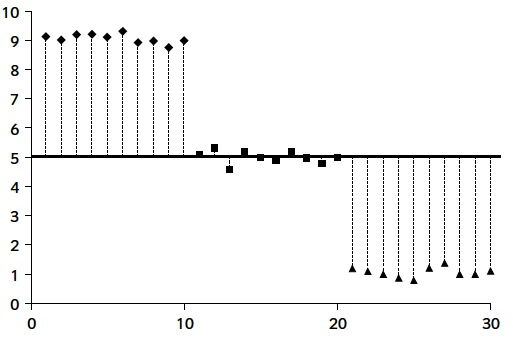
\includegraphics[width=0.8\linewidth]{FD1-1}\\
Molta variabilitat global\ldots 
\end{center}
\end{frame}

\begin{frame}
\frametitle{ANO\ldots VA?}

\begin{center}
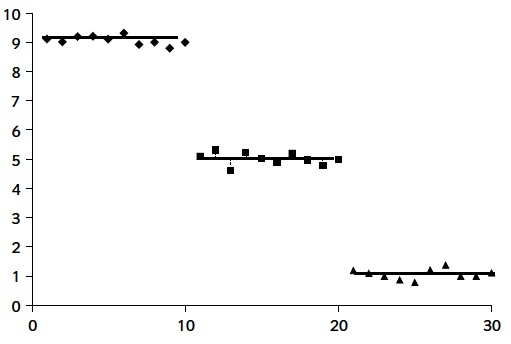
\includegraphics[width=0.8\linewidth]{FD1-2}\\
\ldots\ i molt poca dins cada nivell \\ \pause
\medskip

\red{Evidència que les mitjanes són  diferents}

\end{center}
\end{frame}


\begin{frame}
\frametitle{ANO\ldots VA?}

\begin{center}
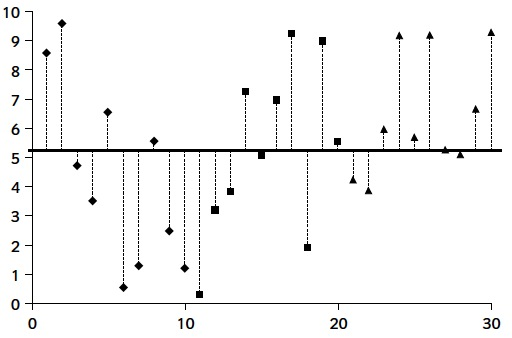
\includegraphics[width=0.8\linewidth]{FD2-1}\\
Molta variabilitat global\ldots 
\end{center}
\end{frame}

\begin{frame}
\frametitle{ANO\ldots VA?}

\begin{center}
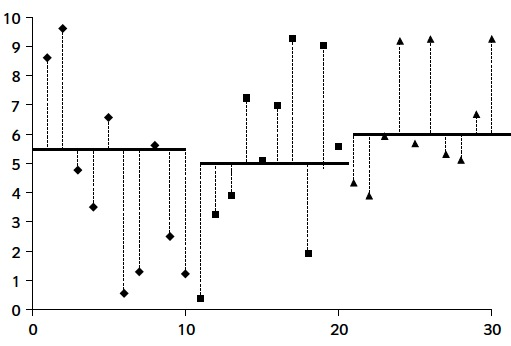
\includegraphics[width=0.8\linewidth]{FD2-2}\\
\ldots\ però també molta dins cada nivell\\ \pause
\medskip

\red{No hi ha evidència que les mitjanes siguin diferents}
\end{center}
\end{frame}

\begin{frame}
\frametitle{ANOVA}\vspace*{-1ex}

En resum: si la suma de les variabilitats dins els nivells és ``suficientment més petita'' que la variabilitat global, serà  evidència  que las mitjanes són diferents\pause\vspace*{-1ex}

\begin{center}
{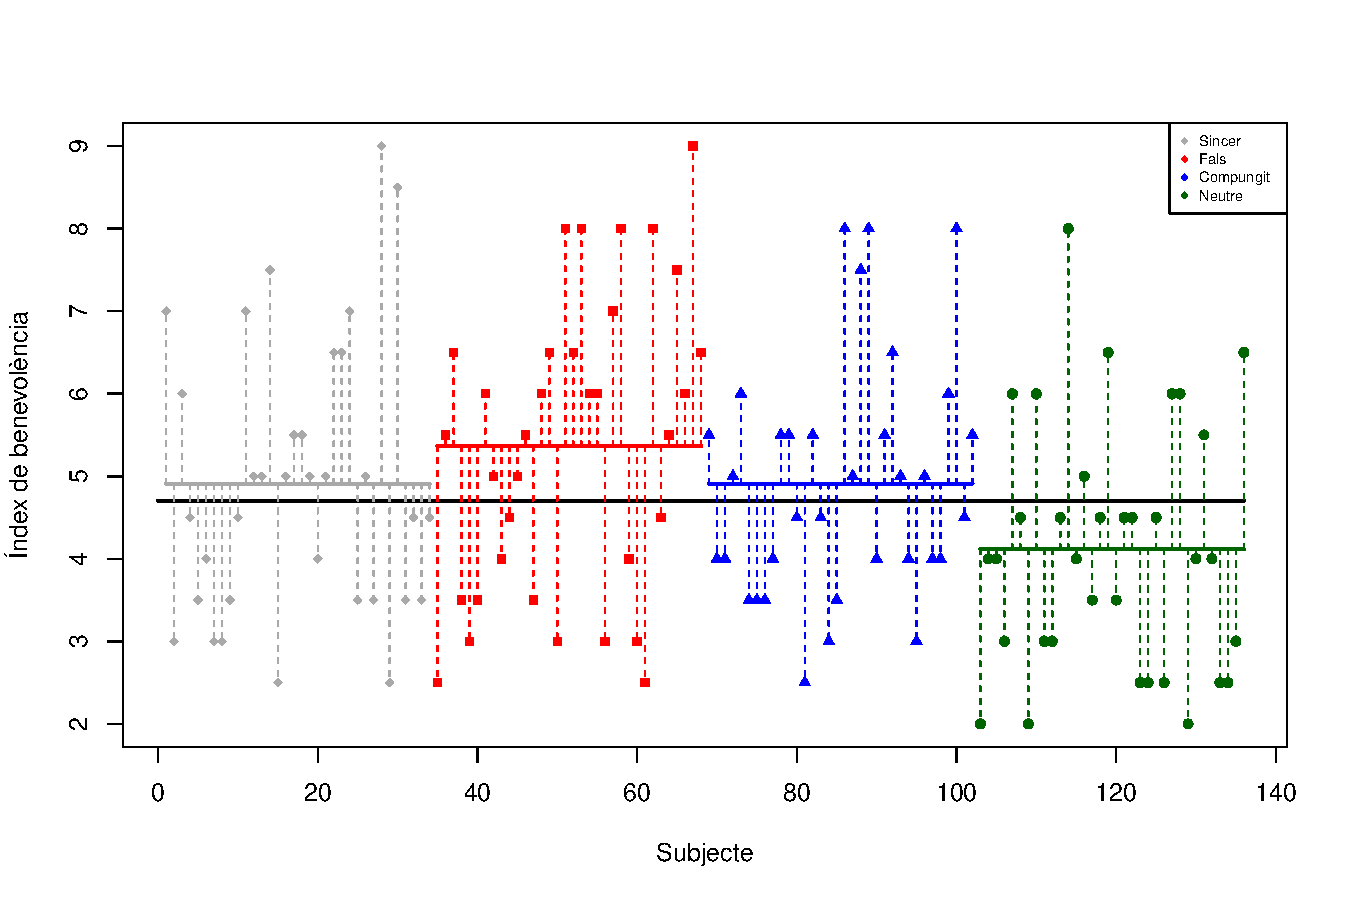
\includegraphics[width=\linewidth]{plotsmilecomplet2}}
\end{center}

\end{frame}



\begin{frame}
\frametitle{Exemple}

Una mostra de 8 resultats de cada, per fer ara a mà:
\begin{center}
\begin{tabular}{cccc}
\multicolumn{4}{c}{Tipus de somriure}\\\hline
Sincer & Fals & Compungit & Neutre\\\hline
6.5 &4.5 &  5.0  &  4.0 \\
4.5 &3.5 & 6.5  &  2.5  \\
4.0 &7.5 & 6.0  &  2.5  \\
7.0  &6.5 & 5.0  &  2.5  \\
5.5 & 3.0 & 5.5  & 2.0  \\
5.0  &3.0 & 3.5  &  5.0  \\
4.5  &5.5 & 4.0  & 2.5  \\
6.0 & 6.0 &5.5  &6.0   
\end{tabular}
\end{center}
\end{frame}


\begin{frame}
\frametitle{Exemple}\vspace*{-2ex}

\begin{center}
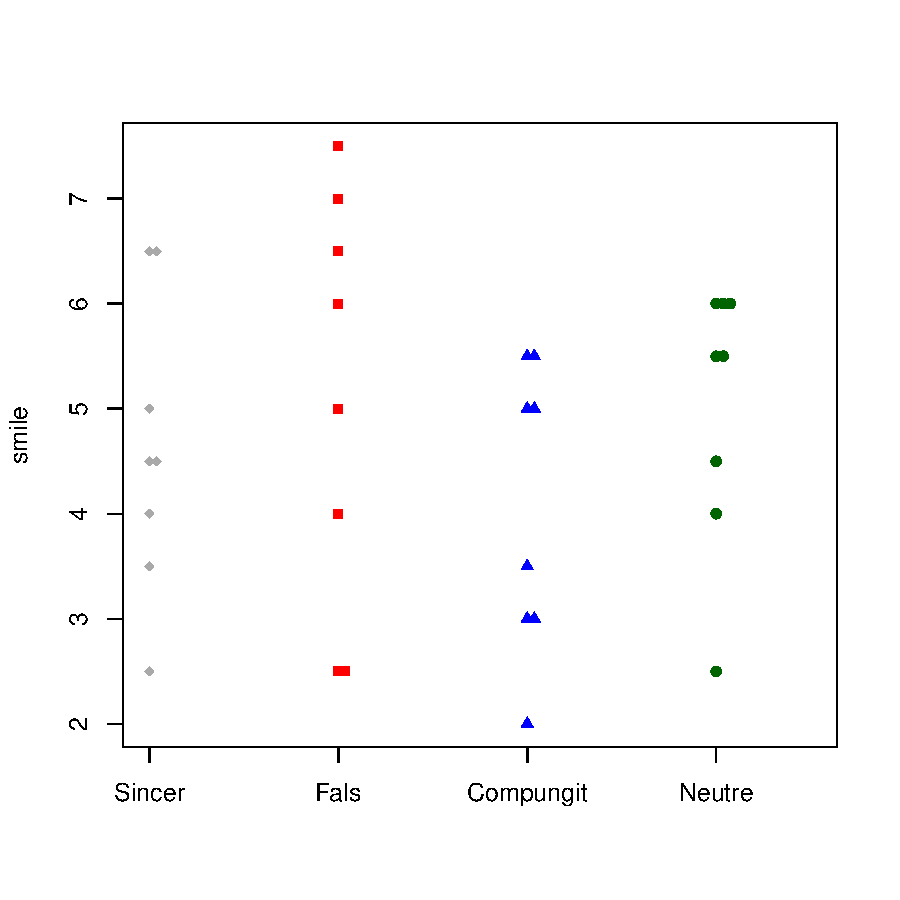
\includegraphics[width=0.8\linewidth]{plotsmile1}
\end{center}

\end{frame}


\begin{frame}
\frametitle{Situació general}

Tenim les dades en una taula:
$$
\begin{array}{c}
\text{Tractaments}\\
\begin{array}{cccc}
 1 & 2 &\ldots & k \\\hline
 X_{11} & X_{21} & \cdots & X_{k1} \\
 X_{12} & X_{22} & \cdots & X_{k2} \\
 \vdots & \vdots & \vdots & \vdots \\
\vdots & \vdots & \vdots & X_{kn_k} \\
X_{1n_1}  & \vdots & \vdots &  \\
 & X_{2n_2} &  &  \\\hline
\end{array}
\end{array}
$$
on 
\begin{itemize}
\item \emph{$n_i$}: mida de la mostra del nivell $i$ (\red{no tenen per què ser iguals}, però  \blue{millor si ho són}: la potència depèn del mínim)\medskip

\item \red{$X_{ij}$}: valor de la característica sota estudi al subjecte $j$ del nivell $i$
\medskip

\end{itemize}
\end{frame}



\begin{frame}
\frametitle{Situació general}\vspace*{-2ex}

\begin{itemize}

\item $\red{N}=n_1+\cdots+n_k$: la mida total de la mostra\smallskip

\item $\red{\overline{X}_{i}}$: Mitjana mostral del nivell $i$-èsim, estima  $\mu_i$
$$ 
\overline{X}_{i}= \frac{\sum_{j=1}^{n_i} X_{ij}}{n_i}
$$


\item $\red{\overline{X}}$: Mitjana mostral de totes les dades, estima $\mu$
$${\overline{X}}=\frac{\sum_{i=1}^k \sum_{j=1}^{n_i} X_{ij}}{N}
$$
\end{itemize}

\begin{center}
\small \begin{tabular}{cccc}
\multicolumn{4}{c}{Nivell del factor}\\\hline
$1$&$2$&$\cdots$&$k$\\\hline
$X_{11}$&$X_{21}$&$\cdots$&$X_{k1}$\\
$X_{12}$&$X_{22}$&$\cdots$&$X_{k2}$\\
$\cdots$&$\cdots$&$\cdots$&$\cdots$\\
$X_{1n_1}$&$X_{2n_2}$&$\cdots$&$X_{kn_k}$\\\hline
$\vphantom{\int^A}\overline{X}_{1}$ &$\overline{X}_{2}$ & $\cdots$&$\overline{X}_{k}$\\[-2ex]
\multicolumn{4}{c}{$\underbrace{\hphantom{\overline{X}_{1}+\overline{X}_{1}+\overline{X}_{1}+\overline{X}_{1}+\overline{X}_{1}}}_{\displaystyle \overline{X}}$}
\end{tabular}
\end{center}

\end{frame}


\begin{frame}
\frametitle{Exemple}


Emmagatzemam les dades de la taula curta en  un \textsl{dataframe} amb dues variables:
\begin{itemize}
\item \texttt{IB}: l'índex de benevolència
\item \texttt{TS}: el tipus de somriure (S,F,C,N)
\end{itemize}

{\begin{center}
\footnotesize \begin{tabular}{cccc}
\multicolumn{4}{c}{Tipus de somriure}\\\hline
Sincer & Fals & Compungit & Neutre\\\hline
6.5 &4.5 &  5.0  &  4.0 \\
4.5 &3.5 & 6.5  &  2.5  \\
4.0 &7.5 & 6.0  &  2.5  \\
7.0  &6.5 & 5.0  &  2.5  \\
5.5 & 3.0 & 5.5  & 2.0  \\
5.0  &3.0 & 3.5  &  5.0  \\
4.5  &5.5 & 4.0  & 2.5  \\
6.0 & 6.0 &5.5  &6.0   
\end{tabular}
\end{center}
}\
\end{frame}


\begin{frame}[fragile]
\frametitle{Exemple}\vspace*{-1ex}

\begin{itemize}
\item \texttt{IB}: l'índex de benevolència
\item \texttt{TS}: el tipus de somriure (S,F,C,N) com a \red{factor}
\end{itemize}

\begin{lstlisting}
> IB=c(6.5,4.5,5.0,4.0,4.5,3.5,6.5,2.5,4.0,7.5,
  6.0,2.5,7.0,6.5,5.0,2.5,5.5,3.0,5.5,2.0,5.0,
  3.0,3.5,5.0,4.5,5.5,4.0,2.5,6.0,6.0,5.5,6.0)
> TS=factor(rep(c("S","F","C","N"),times=8),
          levels=c("S","F","C","N"))
> Benev=data.frame(IB,TS)
> str(Benev)
'data.frame':	32 obs. of  2 variables:
 $ IB: num  6.5 4.5 5 4 4.5 3.5 6.5 2.5 4 7.5 ...
 $ TS: Factor w/ 4 levels "S","F","C","N": 1 2 3 4 1 2 3 4 1 2 ...
> N=dim(Benev)[1]; k=length(levels(Benev$TS))
> c(N,k)
[1] 32 4
\end{lstlisting}
\end{frame}


\begin{frame}[fragile]
\frametitle{Exemple}\vspace*{-1ex}

\begin{itemize}
\item Les $\overline{X}_{i}$:
\end{itemize}
\begin{lstlisting}
> Xb.i=aggregate(IB~TS,data=Benev,mean)
> Xb.i
  TS     IB
1  S 5.3750
2  F 4.9375
3  C 5.1250
4  N 3.3750
\end{lstlisting}

\begin{itemize}
\item La $\overline{X}$:
\end{itemize}
\begin{lstlisting}
> Xb=mean(Benev$IB)
> Xb
[1] 4.703125
\end{lstlisting}


$$
\begin{array}{cccccc}
\overline{X}_s & \overline{X}_f & \overline{X}_c & \overline{X}_n & \quad & \overline{X}\\\hline
5.375 & 4.9375 &  5.125 & 3.375 & & 4.703
\end{array}
$$
\end{frame}



%
%\begin{frame}
%\frametitle{Model}
%$$
%X_{i} -\mu=(X_{i} -\mu_i)+(\mu_i - \mu),\ i=1,\ldots,k,
%$$
%on
%\begin{itemize}
%\item \red{$X_{i}$}: la variable corresponent al nivell $i$-èssim
%\medskip
%
%\item \red{$X_{i}-\mu$}: la desviació del valor de $X_{i}$ en un subjecte respecte de la mitjana global
%\medskip
%
%\item \red{$X_{i}-\mu_i$}: la desviació del valor de $X_{i}$ en un subjecte respecte de la mitjana del seu nivell
%\medskip
%
%\item \red{$\mu_i -\mu$}: desviació de la mitjana del nivell $i$-èsim respecte de la mitjana global 
%\end{itemize}
%\end{frame}
%
%
\begin{frame}
\frametitle{Identitat de les sumes de quadrats}\vspace*{-2ex}

\begin{teorema}
$SS_{Total}=SS_{Tr}+SS_E$
\end{teorema}

on:\vspace*{-2ex}

\begin{itemize}
\item $\red{SS_{Total}}=\sum\limits_{i=1}^k\sum\limits_{j=1}^{n_i} (X_{ij}-\overline{X})^2$; és la \red{Suma Total de Quadrats} i representa la \blue{variabilitat global de la mostra}

\item $\red{SS_{Tr}}=\sum\limits_{i=1}^k n_i
(\overline{X}_{i}-\overline{X})^2$; és la \red{Suma de Quadrats dels Tractaments} i representa la \blue{variabilitat de les mitjanes} 

\item $\red{SS_E}=\sum\limits_{i=1}^k\sum\limits_{j=1}^{n_i} (X_{ij}-\overline{X}_{i})^2$; és la \red{Suma de Quadrats dels Residus} o \red{dels Errors} i representa la \blue{variabilitat dins les mostres}
\end{itemize}\pause

\begin{quote}
\blue{La variabilitat total de la mostra descompon en la suma de les variabilitats de les mostres de cada nivell més la variabilitat de les mitjanes}
\end{quote}

\end{frame}



\begin{frame}[fragile]
\frametitle{Exemple}\vspace*{-3ex}


\begin{itemize}
\item $SS_{Total}=\sum\limits_{i=1}^k\sum\limits_{j=1}^{n_i} (X_{ij}-\overline{X})^2$
\end{itemize}

\begin{lstlisting}
> SSTotal=sum((IB-Xb)^2); SSTotal
[1] 69.42969
\end{lstlisting}\pause

\begin{itemize}
\item $SS_{Tr}=\sum\limits_{i=1}^k n_i
(\overline{X}_{i}-\overline{X})^2$
\end{itemize}

\begin{lstlisting}
> SSTr=sum(table(TS)*(Xb.i[,2]-Xb)^2); SSTr
[1] 19.58594
\end{lstlisting} \pause

\begin{itemize}
\item  $SS_E=\sum\limits_{i=1}^k\sum\limits_{j=1}^{n_i} (X_{ij}-\overline{X}_{i})^2$\pause

\item $SS_E=SS_{Total}-SS_{Tr}$
\end{itemize}

\begin{lstlisting}
> SSE=sum((IB-Xb.i[,2])^2); SSE
[1] 49.84375
> SSTotal-SSTr
[1] 49.84375
\end{lstlisting}
\end{frame}

\begin{frame}
\frametitle{Contrast}

\red{$SS_{Total}=SS_{Tr}+SS_E$}\medskip

Rebutjarem $H_0$ si $SS_{Total}$ és prou més gran que $SS_E$\pause\medskip

Rebutjarem $H_0$ si $SS_{Tr}$ és prou més gran que $SS_E$\pause\medskip

Per mesurar-ho emprarem els estadístics següents:\medskip

\begin{itemize}
\item \emph{Quadrat mitjà dels tractaments}:
$$
\red{MS_{Tr}}=\frac{SS_{Tr}}{k-1}
$$
\item \emph{Quadrat mitjà dels residus} (\red{dels errors}, \red{residual}):
$$
\red{MS_E}=\frac{SS_E}{N-k}
$$
\end{itemize}
i compararem $MS_{Tr}$ amb $MS_E$
\end{frame}


\begin{frame}
\frametitle{Condicions necessàries}

Per poder fer una ANOVA d'1 via, cal que:
\begin{itemize}
\item Les $k$ mostres siguin m.a.s. independents
\medskip

\item $N\geq k+1$\medskip

\item Cadascuna de les $k$ poblacions segueix una llei normal
\medskip

\item \red{Homogeneïtat de les variàncies}, o \red{homocedasticitat}: Totes aquestes poblacions tenen la mateixa variància $\sigma^2$
\end{itemize}\medskip


\emph{No basten mostres grans}: Aquí no juga cap paper el TCL 
\begin{itemize}
\item En general, l'ANOVA és bastant robust contra falta de normalitat

\item però sensible a l'heterocedasticitat
\end{itemize}

\end{frame}

\begin{frame}
\frametitle{Homocedasticitat}

\red{\bf Homocedasticitat}: Totes les subpoblacions tenen la mateixa variància  (\red{\bf NO}: totes les mostres tenen la mateixa variància)

\begin{center}
\blue{Homocedasticitat}\\[1ex]
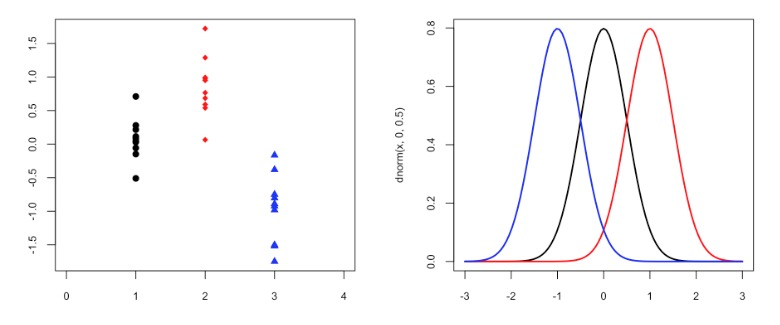
\includegraphics[width=\linewidth]{homoc}
\end{center}

\end{frame}

\begin{frame}
\frametitle{Homocedasticitat}

\red{\bf Homocedasticitat}: Totes les subpoblacions tenen la mateixa variància  (\red{\bf NO}: totes les mostres tenen la mateixa variància)

\begin{center}
\blue{Heterocedasticitat}\\[1ex]
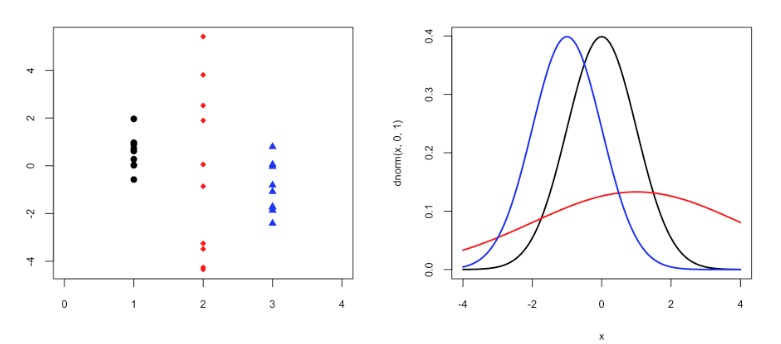
\includegraphics[width=\linewidth]{heteroc}
\end{center}

\end{frame}



\begin{frame}
\frametitle{Contrast}

Si se satisfan les condicions necessàries per fer una ANOVA d'1 via:
\begin{itemize}
\item $E(MS_{Tr})=\displaystyle\sigma^2 + \sum_{i=1}^k \frac{n_i (\mu_i
-\mu)^2}{k-1}$
\medskip

\item $E(MS_E)=\sigma^2$
\end{itemize}
\bigskip

En particular, \red{$MS_E$ és estimador no esbiaixat de la variància comuna $\sigma^2$}
\pause\medskip


Si $H_0:\mu_1=\cdots=\mu_k (=\mu)$ és certa,
$$
\sum_{i=1}^k \frac{n_i (\mu_i -\mu)^2}{k-1}=0,
$$
i si $H_0$ no és certa, aquesta quantitat és $>0$

\end{frame}


\begin{frame}
\frametitle{Contrast}

Per tant
\medskip

\begin{itemize}
\item \red{si $H_0$ és certa}, $E(MS_E)=E(MS_{Tr})$ i hauríem d'esperar que aquests dos estadístics  tinguessin valors propers: que
$$
\red{\frac{MS_{Tr}}{MS_E}\approx 1}
$$
\item \red{si $H_0$ és falsa}, $E(MS_{Tr})>E(MS_E)$ i hauríem d'esperar que 
$$
\red{\frac{MS_{Tr}}{MS_E}> 1}
$$
\end{itemize}
\end{frame}


\begin{frame}
\frametitle{Contrast}

Prenem com a \emph{estadístic de contrast} el quocient 
$$
\red{F=\frac{MS_{Tr}}{MS_E}}
$$
Si $H_0$ és certa i se satisfan les condicions per fer una ANOVA:
\begin{itemize}
\item la seva distribució és $F_{k-1,N-k}$

\smallskip

\item el seu valor serà proper a $1$
\end{itemize}\medskip

A més, si $k=2$, $F$ és igual al quadrat de l'estadístic del test t de 2 mostres independents i variàncies iguals\pause\medskip

\red{Rebutjarem la hipòtesi nu\l.la si $F$ és molt gran}:
$$
\text{p-valor}=P(F_{k-1,N-k}\geq F)
$$



\end{frame}

\begin{frame}
\frametitle{Contrast}

\begin{itemize}
\item Calculam les sumes de quadrats 
$$
SS_{Tr},\ SS_E
$$

\item Calculam 
$$
\hspace*{-5ex} MS_{Tr}=\frac{SS_{Tr}}{k-1},\
MS_E=\frac{SS_E}{N-k},\ F=\frac{MS_{Tr}}{MS_E}
$$

\item Calculam el p-valor
$$
P(F_{k-1,N-k}\geq F)
$$

\item Si el p-valor és més petit que el nivell de significació $\alpha$  rebutjam $H_0$ i concloem que no totes les mitjanes són iguals. En cas contrari, acceptam $H_0$.
\end{itemize}
\end{frame}


\begin{frame}
\frametitle{Contrast}

\begin{center}
\hspace*{-0.5cm}\begin{tabular}{cccc}

\includegraphics[width=0.14\linewidth]{felt} & 

\includegraphics[width=0.15\linewidth]{false} & 

\includegraphics[width=0.125\linewidth]{miserable} & 

\includegraphics[width=0.15\linewidth]{neutral}\\
Sincer & Fals & Compungit & Neutre
\end{tabular}
\end{center}
$$
N=32,\ k=4,\ SS_{Total}=69.43,\ SS_{Tr}=19.586,\ SS_E=49.844
$$

\begin{itemize}
\item Calculam 
$$
\hspace*{-5ex} MS_{Tr}=\frac{SS_{Tr}}{k-1},\
MS_E=\frac{SS_E}{N-k},\ F=\frac{MS_{Tr}}{MS_E}
$$\pause

$$
\begin{array}{c}
MS_{Tr}=\dfrac{19.586}{3}=6.5286,\ 
MS_E=\dfrac{49.844}{18}=1.7801\\
F=\dfrac{6.5286}{1.7801}=3.6675
\end{array}
$$
\end{itemize}
\end{frame}


\begin{frame}
\frametitle{Contrast}

\begin{center}
\hspace*{-0.5cm}\begin{tabular}{cccc}

\includegraphics[width=0.14\linewidth]{felt} & 

\includegraphics[width=0.15\linewidth]{false} & 

\includegraphics[width=0.125\linewidth]{miserable} & 

\includegraphics[width=0.15\linewidth]{neutral}\\
Sincer & Fals & Compungit & Neutre
\end{tabular}
\end{center}
$$
N=32,\ k=4,\ SS_{Total}=69.43,\ SS_{Tr}=19.586,\ SS_E=49.844
$$

\begin{itemize}


\item p-valor: $P(F_{k-1,N-k}\geq F)$
$$
P(F_{3,18}\geq 3.6675) =\texttt{1-1-pf(3.6675,3,18)}=0.024
$$\pause\vspace*{-2ex}

\item Hem obtingut evidència estadística que els nivells de benevolència mitjans per als diferents tipus de somriure no són tots iguals (ANOVA, p-valor 0.024)
\end{itemize}
\end{frame}



\begin{frame}
\frametitle{Taula ANOVA}

Un contrast ANOVA es resumeix en una \red{taula ANOVA}:
{\footnotesize \begin{center}
\hspace*{-3ex}
\begin{tabular}{ll@{}@{}l@{}@{}l@{}l@{}l}
\hline
Origen&Graus&\hspace*{0.6ex} Sumes de&\hspace*{1ex} Quadrats&\hspace*{1ex} Estadístic de&\hspace*{1ex} p-valor\\
Variació&llibertat&\multicolumn{1}{c}{quadrats}&\hspace*{1ex} mitjans&\hspace*{1ex} contrast\\\hline
Nivells \vphantom{$\displaystyle \int$} &$k-1$&\hspace*{1ex} $SS_{Tr}$&\hspace*{1ex} $MS_{Tr}$&\hspace*{2ex}$F$&\hspace*{1ex} p-valor \\[1ex]
Residus&$N-k$&\hspace*{1 ex} $SS_E$&\hspace*{1ex} $MS_E$&\\\hline
\end{tabular}
\end{center}}
\pause\medskip

\blue{Exemple}:
{\footnotesize \begin{center}
\begin{tabular}{ll@{}@{}l@{}@{}l@{}l@{}l}
\hline
Origen&Graus&\hspace*{0.6ex} Sumes de&\hspace*{1ex} Quadrats&\hspace*{1ex} Estadístic de & \hspace*{1ex} p-valor\\
Variació&llibertat&\multicolumn{1}{c}{quadrats}&\hspace*{1ex} mitjans&\hspace*{1ex} contrast\\\hline
Nivells \vphantom{$\displaystyle \int$} &3&\hspace*{1ex} 19.586 &\hspace*{1ex} 6.53 &\hspace*{2ex} 3.67 & \hspace*{1ex} 0.024 \\[1ex]
Residus&28&\hspace*{1 ex} 49.844&\hspace*{1ex} 1.78 &\\\hline
\end{tabular}
\end{center}}\medskip

$M_{S_E}$ estima la variància comuna de les subpoblacions
\end{frame}


\begin{frame}[fragile]
\frametitle{Amb R} 

\begin{lstlisting}
> summary(aov(IB~TS,data=Benev))
            Df Sum Sq Mean Sq F value Pr(>F)  
TS           3  19.59   6.529   3.668  0.024 *
Residuals   28  49.84   1.780                 
------
Signif. codes:  0 `***' 0.001 `**' 0.01 `*' 0.05 `.' 0.1 ` ' 1
\end{lstlisting}

\begin{lstlisting}
> summary(aov(Benev$IB~Benev$TS))
            Df Sum Sq Mean Sq F value Pr(>F)  
Benev$TS     3  19.59   6.529   3.668  0.024 *
Residuals   28  49.84   1.780                 
---------
Signif. codes:  0 `***' 0.001 `**' 0.01 `*' 0.05 `.' 0.1 ` ' 1
\end{lstlisting}\medskip


El valor de {\tt Pr(> F)} és el p-valor del contrast
\end{frame}



\begin{frame}
\frametitle{Podíem aplicar una ANOVA d'1 via?}\vspace*{-3ex}

Per poder fer una ANOVA d'1 via cal que:\medskip

\begin{enumerate}
\item Les mostres de cada nivell són aleatòries simples i independents i $N\geq k+1$\pause
\medskip

\item La població definida per cada nivell ha de ser normal.\pause\ \blue{$\Rightarrow$ Contrastos de normalitat}
\pause\medskip

\item Totes aquestes poblacions han de tenir la mateixa variància\pause\ \blue{$\Rightarrow$ Contrast d'homocedasticitat} 
\end{enumerate}
\end{frame}

\begin{frame}[fragile]
\frametitle{Podíem aplicar una ANOVA d'1 via?}\vspace*{-3ex}

\blue{Contrastos de normalitat}: Triau el més adient en funció de les dades\medskip

\begin{lstlisting}
> shapiro.test(IB[TS=="S"])$p.value
[1] 0.7357702
> shapiro.test(IB[TS=="F"])$p.value
[1] 0.4697832
> shapiro.test(IB[TS=="C"])$p.value
[1] 0.7704917
> shapiro.test(IB[TS=="N"])$p.value
[1] 0.03766128
\end{lstlisting}
\end{frame}

\begin{frame}[fragile] 
\frametitle{Podíem aplicar una ANOVA d'1 via?}\vspace*{-3ex}

\blue{Contrast d'homocedasticitat}:

\begin{itemize}
\item Si les vv.aa. són normals, el millor és el \red{test de Bartlett}: funció \red{\tt bartlett.test}
\end{itemize}
\begin{lstlisting}
> bartlett.test(IB~TS,data=Benev)

	Bartlett test of homogeneity of variances

data:  IB by TS
Bartlett's K-squared = 2.5933, df = 3, p-value = 0.4587
\end{lstlisting}
\medskip

Podríem acceptar que tenen les variàncies iguals
\end{frame}

\begin{frame}[fragile] 
\frametitle{Podíem aplicar una ANOVA d'1 via?}\vspace*{-3ex}

\blue{Contrast d'homocedasticitat}:

\begin{itemize}
\item Si les vv.aa. no són normals, el millor és el \red{test de Fligner-Killeen}: funció \red{\tt fligner.test} 
\end{itemize}
\begin{lstlisting}
> fligner.test(IB~TS,data=Benev)

	Fligner-Killeen test of homogeneity of variances

data:  IB by TS
Fligner-Killeen:med chi-squared = 3.4352, 
df = 3, p-value = 0.3293
\end{lstlisting}
\medskip

Podem acceptar que tenen les variàncies iguals
\end{frame}


\begin{frame}[fragile] 
\frametitle{Contrast no paramètric}

Si no podem emprar una ANOVA d'1 via, hem d'emprar un test no paramètric\medskip

El més popular es el \red{test de Kruskal-Wallis}, que generalitza el test de Mann-Whitney a més de 2 poblacions igual que ANOVA generalitza el test t

\begin{lstlisting}
> kruskal.test(IB~TS,data=Benev)     

	Kruskal-Wallis rank sum test

data:  IB by TS
Kruskal-Wallis chi-squared = 7.8813, df = 3, 
p-value = 0.04853
\end{lstlisting}\medskip


\red{Conclusió}: Hem obtingut evidència estadística que els nivells de benevolència mitjans per als diferents tipus de somriure no són tots iguals (test de Kruskal-Wallis, p-valor 0.0485)

\end{frame}



\begin{frame}[fragile]
\frametitle{Exemple complet}

Les dades completes de l'experiment del somriure són a  \blue{\url{https://raw.githubusercontent.com/AprendeR-UIB/MatesIIAD/master/dades/smiles.txt}}\medskip


\begin{lstlisting}
> Benev.compl=read.table("https://raw.githubusercontent.com/AprendeR-UIB/MatesIIAD/master/dades/smiles.txt",header=TRUE)
> str(Benev.compl)
'data.frame':	136 obs. of  2 variables:
 $ smile   : chr  "felt" "felt" "felt" "felt" ...
 $ leniency: num  7 3 6 4.5 3.5 4 3 3 3.5 4.5 ...
\end{lstlisting}
\end{frame}



\begin{frame}[fragile]
\frametitle{Exemple complet}\vspace*{-1ex}

\begin{lstlisting}
> boxplot(leniency~smile,data=Benev.compl)
\end{lstlisting}\vspace*{-1ex}

\begin{center}
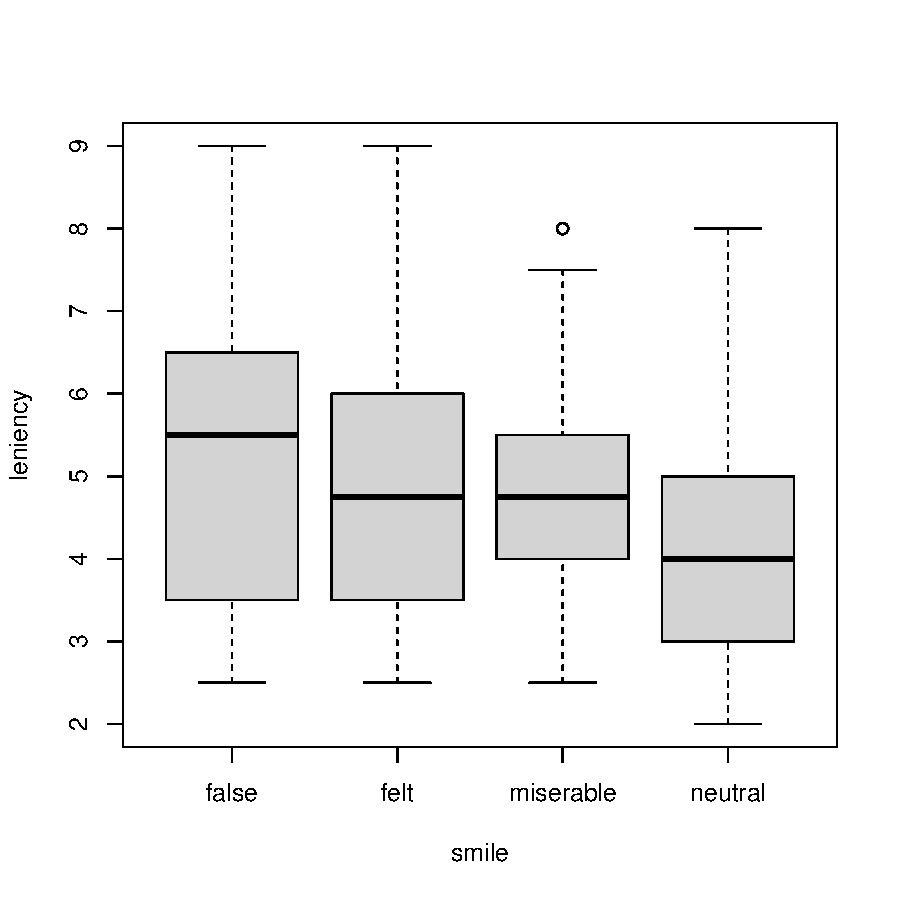
\includegraphics[width=0.8\linewidth]{boxplot}
\end{center}

\end{frame}


\begin{frame}[fragile]
\frametitle{Exemple complet}

\begin{lstlisting}
> shapiro.test(Benev.compl$leniency[Benev.compl$smile=="felt"])$p.value
[1] 0.06464362
> shapiro.test(Benev.compl$leniency[Benev.compl$smile=="false"])$p.value
[1] 0.14510337
> shapiro.test(Benev.compl$leniency[Benev.compl$smile=="miserable"])$p.value
[1] 0.02671712
> shapiro.test(Benev.compl$leniency[Benev.compl$smile=="neutral"])$p.value
[1] 0.07334684
\end{lstlisting}
\end{frame}

\begin{frame}[fragile]
\frametitle{Exemple complet}

\begin{lstlisting}
> fligner.test(leniency~smile,data=Benev.compl)

	Fligner-Killeen test of homogeneity of variances

data:  leniency by smile
Fligner-Killeen:med chi-squared = 3.1294, 
df = 3, p-value = 0.3721
\end{lstlisting}
\end{frame}


\begin{frame}[fragile]
\frametitle{Exemple complet}

\begin{lstlisting}
> summary(aov(leniency~smile,data=Benev.compl))
             Df Sum Sq Mean Sq F value Pr(>F)  
smile         3   27.5   9.178   3.465 0.0182 *
Residuals   132  349.7   2.649                 
\end{lstlisting}\medskip

\red{Conclusió}: Hem obtingut evidència estadística que els nivells de benevolència mitjans per als diferents tipus de somriure no són tots iguals (ANOVA, p-valor 0.018)
\end{frame}

\begin{frame}[fragile]
\frametitle{Exemple complet}

\begin{lstlisting}
> kruskal.test(leniency~smile,data=Benev.compl)  

	Kruskal-Wallis rank sum test

data:  leniency by smile
Kruskal-Wallis chi-squared = 9.1747, df = 3, 
p-value = 0.02706
\end{lstlisting}\medskip

\red{Conclusió}: Hem obtingut evidència estadística que els nivells de benevolència mitjans per als diferents tipus de somriure no són tots iguals (test de Kruskal-Wallis, p-valor 0.027)
\end{frame}


\begin{frame}
\frametitle{I ara què?}\pause

Si hem rebutjat la hipòtesi nul·la $H_0:\mu_1=\cdots =\mu_k$, podem demanar-nos
quins són els nivells diferents
\medskip

Es pot fer de diverses maneres, aquí veurem la més ``òbvia'': comparar totes les parelles de mitjanes per mitjà de tests t 
\end{frame}

\begin{frame}
\frametitle{Comparacions posteriors per parelles} 

Es realitzen els $\binom{k}{2}$
contrastos de 2 mitjanes amb mostres independents i variàncies iguals
$$
\left.
\begin{array}{ll}
H_0 &: \mu_i=\mu_j \\
H_1 &: \mu_i\not=\mu_j
\end{array}
\right\}
$$
\only<2>{\red{Però ara no empram l'estadístic 
$$
T_{i,j}=\frac{\overline{X}_i-\overline{X}_j}{\sqrt{\big(\frac{1}{n_i}+\frac{1}{n_j}\big)\cdot 
\frac{(n_i-1)\widetilde{S}_i^2+(n_j-1)\widetilde{S}_j^2}{n_i+n_j-2}}}
$$
que, si $\mu_i=\mu_j$, té distribució  $t_{n_i+n_j-2}$}}
\only<3,4>{Ara empram l'estadístic
$$
T_{i,j}=\frac{\overline{X}_{i} - \overline{X}_{j}}{\sqrt{\big(\frac{1}{n_i}
+\frac{1}{n_j}\big)\cdot\blue{MS_E} }}
$$
que, $\mu_i=\mu_j$, té distribució $t_{N-k}$}
\medskip

\only<4>{El p-valor de cada contrast és $2P(t_{N-k}\geq |T_{i,j,0}|)$, on $T_{i,j,0}$ és el valor que pren $T_{i,j}$ a la nostra mostra}
\end{frame}



\begin{frame}
\frametitle{\red{Alerta!}}

Si es realitzen $c$ contrastos a un nivell de significació $\alpha$, la probabilitat d'\red{algun} Error de Tipus I  és més gran que $\alpha$: de fet, és \red{$1-(1-\alpha)^c$}
\bigskip

Al nostre \blue{exemple}, si realitzam els 6 contrastos 
$$
\mu_s\stackrel{?}{=}\mu_f,\ \mu_s\stackrel{?}{=}\mu_c,\ \mu_s\stackrel{?}{=}\mu_n,\ 
\mu_f\stackrel{?}{=}\mu_c,\ \mu_f\stackrel{?}{=}\mu_n,\ \mu_c\stackrel{?}{=}\mu_n
$$
amb nivell de significació $\alpha =0.05$,  la probabilitat d'Error de Tipus I a qualcun és 
$ 1-(1-0.05)^{6} \approx 0.265$.
\pause\bigskip

Haurem de reduir el nivell de significació de cada contrast perquè la probabilitat de cometre \red{algun} Error de Tipus I sigui $\alpha$\medskip

O, equivalentement, augmentar (\red{ajustar}) el p-valor de
cada contrast i comparar-lo amb l'$\alpha$ fixat
\end{frame}


\begin{frame}
\frametitle{Ajust de Bonferroni} 

No és el millor, però és el més popular\medskip

Emprant que $1-(1-x)^c \leq c\cdot x$, si volem efectuar $c$ contrastos amb nivell de significació (global) $\alpha$, 
\begin{itemize}
\item \red{realitzam cada contrast amb nivell de significació $\alpha/c$} (i així el nivell de significació 
global serà $\leq c\cdot \alpha/c=\alpha$)\medskip

o equivalentment\medskip

\item \red{multiplicam el p-valor de cada contrast per $c$}
abans de comparar-lo amb el nivell de significació $\alpha$
$$
p<\alpha/c \Longleftrightarrow c\cdot p<\alpha
$$
\end{itemize}\pause\medskip

\red{Atenció!} Els p-valors volen ser probabilitats: si en ajustar-lo  passa d'1, s'ha de donar com a p-valor ajustat \red{1}
\end{frame}


\begin{frame}
\frametitle{Ajust de Bonferroni} 

Al nostre exemple, si realitzam els  6 contrastos, per obtenir un nivell de significació global  $\alpha =0.05$,\medskip

\begin{itemize}
\item  efectuam cada contrast amb nivell de significació
\red{$0.05/6=0.0083$} \medskip

o \medskip

\item multiplicam cada p-valor per \red{6}
\end{itemize}

\end{frame}



\begin{frame}[fragile]
\frametitle{Ajust de Bonferroni} 

Aplicam la funció \red{\texttt{pairwise.t.test}} a la variable numérica i el factor, en aquest ordre, i amb el paràmetre \blue{\texttt{p.adjust.method}} per indicar el mètode d'ajust.\medskip

\begin{itemize}
\item \texttt{p.adjust.method="none"}: no els ajusta
\item \texttt{p.adjust.method="bonferroni"}: ajust de Bonferroni
\item Valor per defecte: mètode de Holm (el millor)
\end{itemize}

\end{frame}


\begin{frame}[fragile]
\frametitle{Ajust de Bonferroni} 

P-valors ``reals'', els hauríem de comparar amb $\alpha/6$\medskip


\begin{lstlisting}
> pairwise.t.test(Benev$IB, Benev$TS,
  p.adjust.method="none") 

Pairwise comparisons using t tests with pooled SD 

data:  Benev$IB and Benev$TS 

  S      F      C     
F 0.5173 -      -     
C 0.7107 0.7807 -     
N 0.0056 0.0265 0.0139

P value adjustment method: none 
\end{lstlisting}

L'únic p-valor per davall de $0.05/6=0.0083$ és el de (S,N)
\end{frame}


\begin{frame}[fragile]
\frametitle{Ajust de Bonferroni} 

P-valors ajustats segons Bonferroni, els hauríem de comparar amb $\alpha$\medskip

\begin{lstlisting}
> pairwise.t.test(Benev$IB, Benev$TS,
  p.adjust.method="bonferroni") 

Pairwise comparisons using t tests with pooled SD 

data:  Benev$IB and Benev$TS 

  S     F     C    
F 1.000 -     -    
C 1.000 1.000 -    
N 0.034 0.159 0.084

P value adjustment method: bonferroni 
\end{lstlisting}\medskip

L'únic p-valor per davall de $0.05$ és el de (S,N)
\end{frame}


\begin{frame}
\frametitle{Conclusió} 

Hem obtingut evidència estadística que els índexos mitjans de benevolència quan  la foto mostra un somriure sincer i quan la foto és neutra són diferents, i no podem rebutjar la igualtat de cap altra parella d'índexos de benevolència mitjans (ANOVA d'1 via, test posterior per parelles de Bonferroni). 
\medskip

\begin{center}
\begin{tabular}{cccc}

\includegraphics[width=0.19\linewidth]{felt} & 

\includegraphics[width=0.21\linewidth]{false} & 

\includegraphics[width=0.173\linewidth]{miserable} & 

\includegraphics[width=0.2\linewidth]{neutral}\\
Sincer & Fals & Compungit & Neutre
\end{tabular}
\end{center}
\end{frame}


\begin{frame}[fragile]
\frametitle{El problema de les comparacions múltiples}\vspace*{-2ex}
\begin{lstlisting}
> shapiro.test(IB[TS=="S"])$p.value
[1] 0.7357702
> shapiro.test(IB[TS=="F"])$p.value
[1] 0.4697832
> shapiro.test(IB[TS=="C"])$p.value
[1] 0.7704917
> shapiro.test(IB[TS=="N"])$p.value
[1] 0.03766128
\end{lstlisting}\pause\vspace*{-1.75ex}
\begin{lstlisting}
> round(4*c(0.7357702,0.4697832,0.7704917,
  0.03766128),3)
[1] 2.943 1.879 3.082 0.151
\end{lstlisting}
\pause\vspace*{-1.75ex}
\begin{lstlisting}
> round(p.adjust(
  c(0.7357702,0.4697832,0.7704917,0.03766128),
  method="bonferroni"),3)
[1] 1.000 1.000 1.000 0.151
\end{lstlisting}

Ajustant per Bonferroni, acceptam que les 4 mostres s'ajusten a variables normals

\end{frame}



 

\begin{frame}
\frametitle{Ajust de Holm}


És més potent que Bonferroni, i el mètode per defecte amb R\medskip

\begin{enumerate}
\item Siguin $C_{1},\ldots ,C_{c}$ els contrastos i $P_{1},\ldots ,P_{c}$ els p-valors corresponents
\medskip

\item Ordenam aquests p-valors en ordre creixent $P_{(1)}\leq \cdots\leq P_{(c)}$ i reenumeram consistentment els contrastos $C_{(1)},\ldots, C_{(c)}$
\medskip

\item Per a cada $j=1,\ldots,c$, calculam el \emph{p-valor ajustat} $\widetilde{P}_{(j)}=(c+1-j)P_{(j)}$
\medskip

\item Aleshores rebutjam la hipòtesi nu\l.la als contrastos $C_{(j)}$ on $\widetilde{P}_{(j)}<\alpha$
 \end{enumerate}


\end{frame}



\begin{frame}
\frametitle{Ajust de Holm}


Fem a mà el mètode de Holm al nostre \blue{exemple}:\medskip

\blue{1)} Taula amb els p-valors dels contrastos

\begin{center}
\begin{tabular}{l|c}
Contrast & p-valor \\ \hline
S-F & 0.5173\\
S-C & 0.7107\\
S-N & 0.0056\\
F-C &0.7807\\
F-N & 0.0265\\
C-N & 0.0139
\end{tabular}
\end{center}

\end{frame}


\begin{frame}
\frametitle{Ajust de Holm}


\blue{2)} Ordenam en ordre creixent del p-valor

\begin{center}
\begin{tabular}{l|c}
Contrast & p-valor \\ \hline
S-N & 0.0056\\
C-N & 0.0139\\
F-N & 0.0265\\
S-F & 0.5173\\
S-C & 0.7107\\
F-C &0.7807\\
\end{tabular}
\end{center}

\end{frame}


\begin{frame}
\frametitle{Ajust de Holm}

\blue{3)} Ajustam: multiplicam el $j$-èsim p-valor per $6+1-j$

\begin{center}
\begin{tabular}{l|cc}
Contrast & p-valor & p-valor ajustat\\ \hline
S-N & 0.0056 & $6\times 0.0056=0.0336 $\\
C-N & 0.0139& $5\times 0.0139=0.0695 $\\
F-N & 0.0265& $4\times 0.0265=0.1060 $\\
S-F & 0.5173& $3\times 0.5173=1.5519 $\\
S-C & 0.7107& $2\times 0.7107=1.4214 $\\
F-C &0.7807& $1\times 0.7807=0.7807$\\
\end{tabular}
\end{center}
\end{frame}

\begin{frame}
\frametitle{Ajust de Holm}

\blue{3)} Ajustam: multiplicam el $j$-èsim p-valor per $6+1-j$

\begin{center}
\begin{tabular}{l|cc}
Contrast & p-valor & p-valor ajustat\\ \hline
S-N & 0.0056 & $6\times 0.0056=0.0336 $\\
C-N & 0.0139& $5\times 0.0139=0.0695 $\\
F-N & 0.0265& $4\times 0.0265=0.1060 $\\
S-F & 0.5173& $3\times 0.5173=\blue{1}\hphantom{.5519} $\\
S-C & 0.7107& $2\times 0.7107=\blue{1}\hphantom{.5519} $\\
F-C &0.7807& $1\times 0.7807=0.7807$\\
\end{tabular}
\end{center}
\end{frame}


\begin{frame}
\frametitle{Ajust de Holm}

\blue{4)} Miram els p-valors per davall del nivell de significació $\alpha$

\begin{center}
\begin{tabular}{l|cc}
Contrast & p-valor & p-valor ajustat\\ \hline
S-N & 0.0056 & $6\times 0.0056=\red{0.0336} $\\
C-N & 0.0139& $5\times 0.0139=0.0695 $\\
F-N & 0.0265& $4\times 0.0265=0.1060 $\\
S-F & 0.5173& $3\times 0.5173=1\hphantom{.5519} $\\
S-C & 0.7107& $2\times 0.7107=1\hphantom{.5519} $\\
F-C &0.7807& $1\times 0.7807=0.7807$\\
\end{tabular}
\end{center}

Mateixa conclusió que amb Bonferroni: concloem que $\mu_S\neq \mu_N$  i no podem rebutjar que les altres parelles de mitjanes siguin iguals

\end{frame}




\begin{frame}[fragile]
\frametitle{Ajust de Holm}

\begin{lstlisting}
> pairwise.t.test(Benev$IB,Benev$TS)  
  #o p.adjust.method="holm"

	Pairwise comparisons using t tests with pooled SD 

data:  Benev$IB and Benev$TS 

  S     F     C    
F 1.000 -     -    
C 1.000 1.000 -    
N 0.034 0.106 0.070
\end{lstlisting}

\end{frame}

\begin{frame}[fragile]
\frametitle{Tests posteriors no paramètrics}\vspace*{-1ex}

Si no té sentit emprar tests t amb variàncies iguals, podem fer contrastos per parelles de Mann-Whitney amb
\begin{lstlisting}
pairwise.wilcox.test(..., paired=FALSE,
   p.adjust.method=...)
\end{lstlisting}\pause

\begin{lstlisting}
> pairwise.wilcox.test(Benev$IB,Benev$TS,
  paired=FALSE, p.adjust.method="bonferroni")

	Pairwise comparisons using Wilcoxon rank sum test with continuity correction 

data:  Benev$IB and Benev$TS 

  S    F    C   
F 1.00 -    -   
C 1.00 1.00 -   
N 0.12 0.26 0.18

P value adjustment method: bonferroni
\end{lstlisting}

\end{frame}

\begin{frame}[fragile]
\frametitle{Exemple complet} 

Les dades completes de l'experiment del somriure són a  \blue{\url{https://raw.githubusercontent.com/AprendeR-UIB/MatesIIAD/master/dades/smiles.txt}}\medskip


\begin{lstlisting}
> Benev.compl=read.table("https://raw.githubusercontent.com/AprendeR-UIB/MatesIIAD/master/dades/smiles.txt",header=TRUE)
> str(Benev.compl)
'data.frame':	136 obs. of  2 variables:
 $ smile   : chr  "felt" "felt" "felt" "felt" ...
 $ leniency: num  7 3 6 4.5 3.5 4 3 3 3.5 4.5 ...
> boxplot(leniency~smile,data=Benev.compl)
\end{lstlisting}
\end{frame}


\begin{frame}
\frametitle{Exemple complet} \vspace*{-2ex}


\begin{center}
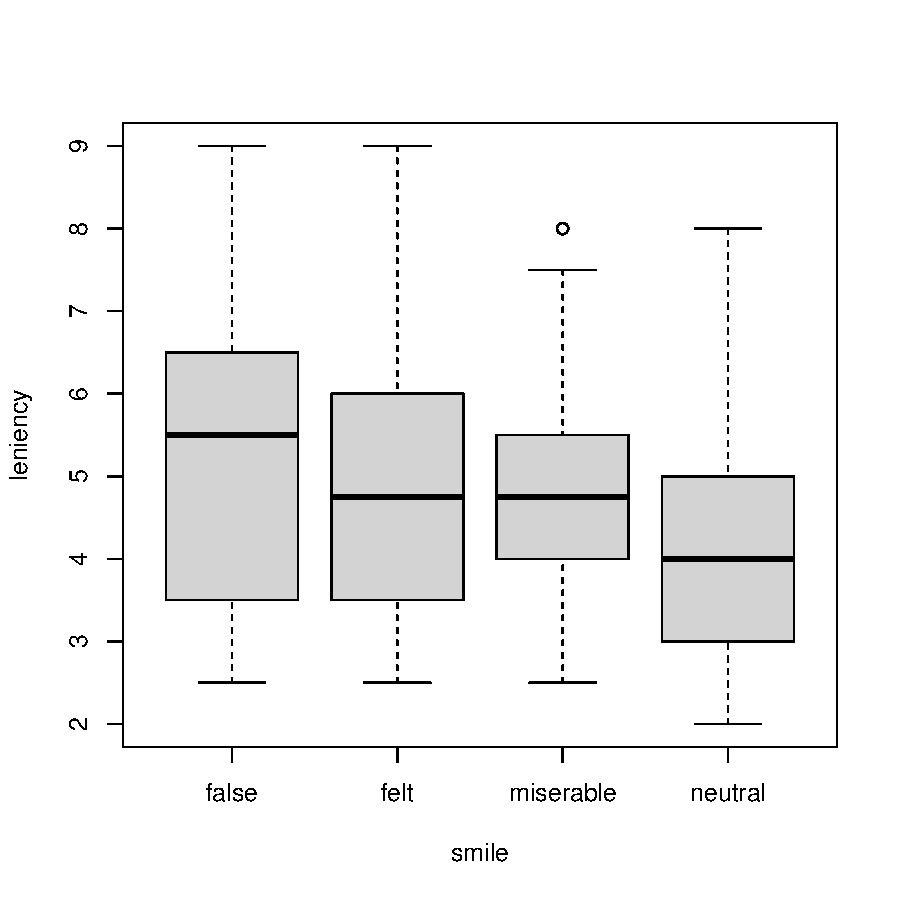
\includegraphics[width=0.8\linewidth]{boxplot}
\end{center}
\end{frame}


\begin{frame}[fragile]
\frametitle{Exemple complet} 

\begin{lstlisting}
> pairwise.t.test(Benev.compl$leniency,Benev.compl$smile,p.adjust.method="bonferroni") 

	Pairwise comparisons using t tests with pooled SD 

data:  Benev.compl$leniency and Benev.compl$smile 

          false felt  miserable
felt      1.000 -     -        
miserable 1.000 1.000 -        
neutral   0.011 0.278 0.278    

P value adjustment method: bonferroni 
\end{lstlisting}
\end{frame}

\begin{frame}[fragile]
\frametitle{Exemple complet} 

\begin{lstlisting}
> pairwise.t.test(Benev.compl$leniency,Benev.compl$smile) 

	Pairwise comparisons using t tests with pooled SD 

data:  Benev.compl$leniency and Benev.compl$smile 

          false felt  miserable
felt      0.751 -     -        
miserable 0.751 1.000 -        
neutral   0.011 0.231 0.231    

P value adjustment method: holm 
\end{lstlisting}
\end{frame}

\begin{frame}[fragile]
\frametitle{Exemple complet}\vspace*{-1ex}

\begin{lstlisting}
> pairwise.wilcox.test(Benev.compl$leniency,Benev.compl$smile) 

	Pairwise comparisons using Wilcoxon rank sum test with continuity correction 

data:  Benev.compl$leniency and Benev.compl$smile 

          false felt  miserable
felt      0.802 -     -        
miserable 0.802 0.805 -        
neutral   0.032 0.209 0.209    

P value adjustment method: holm 
\end{lstlisting}\vspace{-1.4ex}

\begin{lstlisting}[style=warning]
Warning messages:
1: In wilcox.test.default(xi, xj, paired = paired, ...) :
  cannot compute exact p-value with ties
\end{lstlisting}
\end{frame}


\end{document}



\subsection{Comparacions per parelles}
\begin{frame}
\frametitle{Comparacions per parelles}

Si hem rebutjat la hipòtesi nul·la $H_0:\mu_1=\cdots =\mu_k$, podem demanar-nos
quins són els nivells diferents
\medskip

Es pot fer de diverses maneres, aquí veurem la més ``òbvia'': comparar totes les parelles de mitjanes per mitjà de tests t 
\end{frame}

\begin{frame}
\frametitle{Comparacions per parelles}
Es realitzen els $\binom{k}{2}$
contrastos
$$
\left.
\begin{array}{ll}
H_0 &: \mu_i=\mu_j \\
H_1 &: \mu_i\not=\mu_j
\end{array}
\right\}
$$
L'estadístic de cada contrast   és ara 
$$
T=\frac{\overline{X}_{i} - \overline{X}_{j}}{\sqrt{\red{MS_E}\cdot (\frac{1}{n_i}
+\frac{1}{n_j})}}
$$
i segueix una distribució $t$ de Student amb $N-k$ graus de
llibertat, $t_{N-k}$
\medskip

El p-valor de cada contrast és $2P(t_{N-k}\geq |t_{i,j}|)$, on $t_{i,j}$ és el valor que hi pren l'estadístic
\end{frame}



\begin{frame}
\frametitle{Comparacions per parelles}
\red{Alerta!}
Si es realitzen $c$ contrastos a un nivell de significació $\alpha$, la probabilitat d'Error de Tipus I a qualcun és més gran que $\alpha$: de fet, és $ 1-(1-\alpha)^c$
\bigskip

Per exemple, a l'exemple del CO${}_2$, si realitzam $c=\binom{5}{2}=10$ contrastos amb nivell de significació $\alpha =0.05$, la probabilitat d'Error de Tipus I a qualcun és 
$ 1-(1-0.05)^{10} \approx 0.4$.
\bigskip

Haurem de reduir el nivell de significació de cada contrast perquè la probabilitat final d'Error de Tipus I sigui $\alpha$\medskip

O, equivalentement, augmentar (\red{ajustar}) el p-valor de
cada contrast i comparar-lo amb l'$\alpha$ fixat
\end{frame}


\begin{frame}
\frametitle{Test T de Bonferroni}

És el més popular\medskip

Emprant l'aproximació $1-(1-x)^c \approx c\cdot x$, si volem efectuar $c$ contrastos amb nivell de significació (global) $\alpha$, 
\begin{itemize}
\item \red{realitzam cada contrast amb nivell de significació $\alpha/c$} (i així el nivell de significació 
global serà $\approx c\cdot \alpha/c=\alpha$)\medskip

o equivalentment\medskip

\item \red{multiplicam el p-valor de cada contrast per $c$}
abans de comparar-lo amb el nivell de significació $\alpha$
$$
p<\alpha/c \Longleftrightarrow c\cdot p<\alpha
$$
\end{itemize}
\end{frame}


\begin{frame}
\frametitle{Test T de Bonferroni}

A l'Exemple 1, si realitzam els  $10$ contrastos, per obtenir un nivell de significació global  $\alpha =0.05$,\medskip

\begin{itemize}
\item  efectuam cada contrast amb nivell de significació
\red{$0.005$}, o \medskip

\item multiplicam cada p-valor per \red{10}
\end{itemize}\bigskip

A l'Exemple 2, si realitzam els  $6$ contrastos, per obtenir un nivell de significació global  $\alpha =0.05$,\medskip

\begin{itemize}
\item  efectuam cada contrast amb nivell de significació
\red{$0.05/6=0.0083$}, o \medskip

\item multiplicam cada p-valor per \red{6}
\end{itemize}



\end{frame}


%
%
%\begin{frame}[fragile]
%\frametitle{Exemple 1}
%$\alpha=0.05$
%\medskip
%
%
%Fem els càlculs per passes
%\medskip
%
%En primer lloc cream una matriu amb fileres les parelles de nivells les mitjanes dels quals contrastarem:
%
% \begin{lstlisting}
%> pars=rbind(c(1,2),c(1,3),c(1,4),c(1,5),
%  c(2,3),c(2,4),c(2,5),c(3,4),c(3,5),c(4,5))
%\end{lstlisting}
%
%\end{frame}
%
%\begin{frame}[fragile]
%\frametitle{Exemple 1}
%
%A continuació calculam els valors  de tots els estadístics de contrast
%\begin{lstlisting}
%> est.par =
% (mitjanes.nivells[pars[,1],2]
%      -mitjanes.nivells[pars[,2],2])/
%  (sqrt(MSE*(1/10+1/10)))
%> est.par
% [1]  5.562226  9.634116 14.296195 18.130310  
% [5] 4.071889  8.733969 12.568084 4.662080  
% [9] 8.496194  3.834115
%\end{lstlisting}
%
%\end{frame}
%
%\begin{frame}[fragile]
%\frametitle{Exemple 1}
%\vspace*{-2ex}
%
%Els afegim com a columna a la matriu de parelles de nivells
%\begin{lstlisting}
%> pars=cbind(pars,est.par)
%> round(pars,4)
%          est.par
% [1,] 1 2  5.5622
% [2,] 1 3  9.6341
% [3,] 1 4 14.2962
% [4,] 1 5 18.1303
% [5,] 2 3  4.0719
% [6,] 2 4  8.7340
% [7,] 2 5 12.5681
% [8,] 3 4  4.6621
% [9,] 3 5  8.4962
%[10,] 4 5  3.8341
%\end{lstlisting}
%
%\end{frame}
%
%\begin{frame}[fragile]
%\frametitle{Exemple 1}
%\vspace*{-2ex}
%
%Calculam els p-valors:
%
%\begin{lstlisting}
%> p.valCO2=function(x){2*(1-pt(abs(x),N-k))}
%> p.vals=sapply(est.par,p.valCO2)
%> p.vals
% [1] 1.387522e-06 1.649791e-12 0.000000e+00
% [4] 0.000000e+00 1.863744e-04 3.021050e-11
% [7] 2.220446e-16 2.808032e-05 6.609646e-11
%[10] 3.892218e-04
%\end{lstlisting}
%
%\end{frame}
%
%\begin{frame}[fragile]
%\frametitle{Exemple 1}
%\vspace*{-2ex}
%
%Ho afegim com a columna a la matriu de parelles de nivells i estadístics
%\begin{lstlisting}
%> pars=cbind(pars,p.vals)
%> round(pars,5)
%           est.par  p.vals
% [1,] 1 2  5.56223 0.00000
% [2,] 1 3  9.63412 0.00000
% [3,] 1 4 14.29620 0.00000
% [4,] 1 5 18.13031 0.00000
% [5,] 2 3  4.07189 0.00019
% [6,] 2 4  8.73397 0.00000
% [7,] 2 5 12.56808 0.00000
% [8,] 3 4  4.66208 0.00003
% [9,] 3 5  8.49619 0.00000
%[10,] 4 5  3.83411 0.00039
%\end{lstlisting}
%
%\end{frame}
%\begin{frame}[fragile]
%\frametitle{Exemple 1}
%\vspace*{-2ex}
%
%\red{\bf Bonferroni}: Quins p-valors són inferiors a 0.005?
%\begin{lstlisting}
%> pars[which(p.vals<0.005),c(1,2)]        
% [1,] 1 2
% [2,] 1 3
% [3,] 1 4
% [4,] 1 5
% [5,] 2 3
% [6,] 2 4
% [7,] 2 5
% [8,] 3 4
% [9,] 3 5
%[10,] 4 5
%\end{lstlisting}
%
%
%Tots. Per tant, rebutjam totes les hipòtesis nu\l.les, i concloem que els nivells tenen mitjanes diferents dues a dues
%
%\end{frame}
%
%\begin{frame}[fragile]
%\frametitle{Exemple 1}
%\vspace*{-2ex}
%
%\red{\bf Holm}: Ordenam les fileres de \texttt{pars} ordenant els p-valors de menor a major:
%\begin{lstlisting}
%> pars.ord=pars[order(pars[,4]),]
%> round(pars.ord,5)
%           est.par  p.vals
% [1,] 1 4 14.29620 0.00000
% [2,] 1 5 18.13031 0.00000
% [3,] 2 5 12.56808 0.00000
% [4,] 1 3  9.63412 0.00000
% [5,] 2 4  8.73397 0.00000
% [6,] 3 5  8.49619 0.00000
% [7,] 1 2  5.56223 0.00000
% [8,] 3 4  4.66208 0.00003
% [9,] 2 3  4.07189 0.00019
%[10,] 4 5  3.83411 0.00039
%\end{lstlisting}
%\end{frame}
%
%
%\begin{frame}[fragile]
%\frametitle{Exemple 1}
%\vspace*{-2ex}
%
%\red{\bf Holm}: Calculam els p-valors ajustats i els afegim com a columna a \texttt{pars.ord} 
%\begin{lstlisting}
%> p.vals.adj=pars.ord[,4]*(10+1-1:10)
%> pars.ord=cbind(pars.ord,p.vals.adj)
%> round(pars.ord,5)
%           est.par  p.vals p.vals.adj
% [1,] 1 4 14.29620 0.00000    0.00000
% [2,] 1 5 18.13031 0.00000    0.00000
% [3,] 2 5 12.56808 0.00000    0.00000
% [4,] 1 3  9.63412 0.00000    0.00000
% [5,] 2 4  8.73397 0.00000    0.00000
% [6,] 3 5  8.49619 0.00000    0.00000
% [7,] 1 2  5.56223 0.00000    0.00001
% [8,] 3 4  4.66208 0.00003    0.00008
% [9,] 2 3  4.07189 0.00019    0.00037
%[10,] 4 5  3.83411 0.00039    0.00039
%\end{lstlisting}
%\end{frame}
%
%
%
%
%\begin{frame}[fragile]
%\frametitle{Exemple 1}
%\vspace*{-2ex}
%
%\red{\bf Holm}: A quins contrastos $C_{(k)}$ tenim que $\widetilde{P}_{k}\leq 0.05$?
%\begin{lstlisting}
%> pars.ord[which(pars.ord[,5]<=0.05),c(1,2)]  
% [1,] 1 4
% [2,] 1 5
% [3,] 2 5
% [4,] 1 3
% [5,] 2 4
% [6,] 3 5
% [7,] 1 2
% [8,] 3 4
% [9,] 2 3
%[10,] 4 5
%\end{lstlisting}
%A tots, per tant rebutjam totes les hipòtesis nu\l.les, i concloem que els nivells tenen mitjanes diferents dues a dues
%
%\end{frame}
%
%
%
%



\begin{frame}[fragile]
\frametitle{Amb R} 

Amb R, per calcular tots els p-valors de cop podem aplicar la funció \red{\texttt{pairwise.t.test}} a la variable numérica i el factor, en aquest ordre, i a \blue{\texttt{p.adjust.method="none"}}\bigskip

Si voleu els p-valors ja ajustats, cal igualar \blue{\texttt{p.adjust.method}} al mètode d'ajust desitjat, per exemple a \blue{\texttt{"bonferroni"}}

\end{frame}


\begin{frame}[fragile]
\frametitle{Exemple 2}\vspace*{-1ex}

P-valors ``reals'', els hauríem de comparar amb $\alpha/6$\medskip


\begin{lstlisting}
> pairwise.t.test(EG$Expr,EG$Tract,
  p.adjust.method="none")

	Pairwise comparisons using t tests with pooled SD 

data:  EG$Expr and EG$Tract 

  A       B       C      
B 0.06554 -       -      
C 0.00756 0.29688 -      
D 0.00058 0.03522 0.23937

P value adjustment method: none
\end{lstlisting}

Els únics p-valors per davall de $0.05/6=0.0083$ són els de (A,C) i (A,D)

\end{frame}


\begin{frame}[fragile]
\frametitle{Exemple 2}\vspace*{-1ex}

P-valors ajustats segons Bonferroni, els hauríem de comparar amb $\alpha$\medskip

\begin{lstlisting}
> pairwise.t.test(EG$Expr,EG$Tract,
  p.adjust.method="bonferroni")
...
  A      B      C     
B 0.3933 -      -     
C 0.0453 1.0000 -     
D 0.0035 0.2113 1.0000

P value adjustment method: bonferroni 
\end{lstlisting}\medskip

Els únics p-valors per davall de 0.05 són (A,C) i (A,D)
\end{frame}

 

\begin{frame}
\frametitle{Test T de Holm}
\vspace*{-1ex}

És més potent que Bonferroni, i el mètode per defecte amb R\medskip

\begin{enumerate}
\item Siguin $C_{1},\ldots ,C_{c}$ els contrastos i $P_{1},\ldots ,P_{c}$ els p-valors corresponents
\medskip

\item Ordenam aquests p-valors en ordre creixent $P_{(1)}\leq \cdots\leq P_{(c)}$ i reenumeram consistentment els contrastos $C_{(1)},\ldots, C_{(c)}$
\medskip

\item Per a cada $j=1,\ldots,c$, calculam el \emph{p-valor ajustat} $\widetilde{P}_{(j)}=(c+1-j)P_{(j)}$
\medskip

\item Aleshores rebutjam la hipòtesi nu\l.la als contrastos $C_{(j)}$ on $\widetilde{P}_{(j)}<\alpha$
 \end{enumerate}


\end{frame}



\begin{frame}
\frametitle{Exemple 2}

Fem a mà el mètode de Holm:\medskip

\blue{1)} Taula amb els p-valors dels contrastos

\begin{center}
\begin{tabular}{l|c}
Contrast & p-valor \\ \hline
A-B & 0.06554\\
A-C & 0.00756\\
A-D & 0.00058\\
B-C &0.29688\\
B-D & 0.03522\\
C-D & 0.23937
\end{tabular}
\end{center}

\end{frame}


\begin{frame}
\frametitle{Exemple 2}

Fem a mà el mètode de Holm:\medskip

\blue{2)} Ordenam en ordre creixent del p-valor

\begin{center}
\begin{tabular}{l|c}
Contrast & p-valor \\ \hline
A-D & 0.00058\\
A-C & 0.00756\\
B-D & 0.03522\\
A-B & 0.06554\\
C-D & 0.23937\\
B-C &0.29688\\
\end{tabular}
\end{center}

\end{frame}


\begin{frame}
\frametitle{Exemple 2}

Fem a mà el mètode de Holm:\medskip

\blue{3)} Ajustam: multiplicam el $j$-èsim p-valor per $6+1-j$

\begin{center}
\begin{tabular}{l|cc}
Contrast & p-valor & p-valor ajustat\\ \hline
A-D & 0.00058 & $6\times 0.00058 = 0.00348$\\
A-C & 0.00756 & $5\times 0.00756 = 0.03780$\\
B-D & 0.03522 & $4\times 0.03522 = 0.14088$\\
A-B & 0.06554 & $3\times 0.06554 =  0.19662$\\
C-D & 0.23937 & $2\times 0.23937 = 0.47874$\\
B-C & 0.29688 & $1\times 0.29688 = 0.29688$\\
\end{tabular}
\end{center}

Mateixa conclusió que amb Bonferroni: concloem que $\mu_A\neq \mu_D$ i $\mu_A\neq \mu_C$, i no podem rebutjar que les altres parelles de mitjanes siguin iguals

\end{frame}




\begin{frame}[fragile]
\frametitle{Exemple 2}

Fent \blue{\texttt{p.adjust.method="holm"}} (o no especificant \blue{\texttt{p.adjust.method}}, ja que és el mètode per defecte) obtenim els p-valors ajustats del mètode de Holm\medskip


\begin{lstlisting}
> pairwise.t.test(EG$Expr,EG$Tract,
  p.adjust.method="holm")
...
  A      B      C     
B 0.1966 -      -     
C 0.0378 0.4787 -     
D 0.0035 0.1409 0.4787

P value adjustment method: holm 
\end{lstlisting}

\end{frame}


\begin{frame}[fragile]
\frametitle{Exemple 1}


\begin{lstlisting}
> pairwise.t.test(CO2$Inc,CO2$Pre,
   p.adjust.method="bonferroni")

...
      0.0      0.08   0.29    0.50   
0.08 1.4e-05 -       -       -      
0.29  1.6e-11 0.00186 -       -      
0.50  < 2e-16 3.0e-10 0.00028 -      
0.86  < 2e-16 2.5e-15 6.6e-10 0.00389

P value adjustment method: bonferroni 
\end{lstlisting}



\end{frame}


\begin{frame}[fragile]
\frametitle{Exemple 1}


\begin{lstlisting}
> pairwise.t.test(CO2$Inc,CO2$Pre,
   p.adjust.method="holm")

...
      0.0     0.08   0.29    0.50   
0.08 5.6e-06 -       -       -      
0.29  1.2e-11 0.00037 -       -      
0.50  < 2e-16 1.8e-10 8.4e-05 -      
0.86  < 2e-16 2.0e-15 3.3e-10 0.00039

P value adjustment method: holm 
\end{lstlisting}



\end{frame}




\subsection{Condicions}

\begin{frame} 
\frametitle{Condicions per a l'ANOVA d'1 via}\vspace*{-2ex}

Perquè la conclusió d'una ANOVA d'1 via tengui sentit:\medskip
\begin{enumerate}
\item Les mostres de cada nivell han de ser aleatòries (simples) i independents i $N\geq k+1$.
\medskip

\item La població definida per cada nivell ha de ser normal. Això es contrasta amb contrastos de normalitat. \medskip

\item Totes aquestes poblacions han de tenir la mateixa variància (\red{homocedasticitat}).
\end{enumerate}
\medskip

(1) és responsabilitat de l'investigador, però (2) i (3) s'han de contrastar\medskip

\red{Si fallen, no es pot usar ANOVA: convé emprar un test no paramètric}
\end{frame}





\begin{frame}[fragile] 
\frametitle{Homocedasticitat}


La manera més popular de comprovar l'homocedasticitat (quan acceptam que les mostres provenen de distribucions normals) és amb el \red{test de Bartlett}, implementat en \texttt{R} en la funció \red{\tt bartlett.test}\medskip

\begin{lstlisting}
> bartlett.test(CO2$Inc~CO2$Pre)

	Bartlett test of homogeneity of variances

data:  CO2$Inc by CO2$Pre
Bartlett's K-squared = 1.0701, df = 4, p-value = 0.899
\end{lstlisting}\medskip

Podem acceptar que tenen les variàncies iguals
\end{frame}


\subsection{No paramètric}



\begin{frame}[fragile] 
\frametitle{Contrast no paramètric}\vspace*{-1ex}

Si en un experiment  d'1 via no podem emprar una ANOVA perquè no se satisfaci la normalitat de les poblacions o l'homocedasticitat, cal emprar un test no paramètric\medskip

El més popular es el \red{test de Kruskal-Wallis}, que generalitza el test de Mann-Whitney a més de 2 poblacions igual que ANOVA generalitza el test t; es fa amb la funció \red{\texttt{kruskal.test}}\medskip


\begin{lstlisting}
> kruskal.test(CO2$Inc~CO2$Pre)

	Kruskal-Wallis rank sum test

data:  CO2$Inc by CO2$Pre
Kruskal-Wallis chi-squared = 44.716, df = 4, p-value = 4.555e-09
\end{lstlisting}


\end{frame}


\begin{frame}
\frametitle{Contrast no paramètric}

Si el test de Kruskal permet rebutjar la igualtat de  \red{\textst{mitjanes}} \red{\underline{medianes}}, i voleu determinar quins parells són diferents,  disposau de la funció \red{\texttt{pairwise.wilcox.test}} que efectua contrastos per parelles de Mann-Whitney (amb \blue{\texttt{paired=FALSE}})\medskip

Té la mateixa sintaxi que \texttt{pairwise.t.test}. El mètode d'ajust dels p-valors s'hi entra amb \blue{\texttt{p.adjust.method}} i per defecte és el de Holm.

\end{frame}


\begin{frame}[fragile] 
\frametitle{Contrast no paramètric}


\begin{lstlisting}
> pairwise.wilcox.test(CO2$Inc, CO2$Pre,
 paired=FALSE, p.adjust.method="bonferroni")
\end{lstlisting}\vspace{-1.4ex}

\begin{lstlisting}[style=warning]
cannot compute exact p-value with ties
\end{lstlisting}\vspace{-1.4ex}

\begin{lstlisting}
	Pairwise comparisons using Wilcoxon rank sum test 

data:  CO2$Inc and CO2$Pre 

      0.0     0.083   0.29    0.50   
0.083 0.00211 -       -       -      
0.29  0.00011 0.01050 -       -      
0.50  0.00011 0.00011 0.00325 -      
0.86  0.00011 0.00011 0.00011 0.03186

P value adjustment method: bonferroni\end{lstlisting}

\end{frame}


\end{document}



\begin{frame}
\frametitle{Contrast no paramètric}

Si el test de Kruskal permet rebutjar la igualtat de  \red{\textst{mitjanes}} \red{\underline{medianes}}, i voleu determinar quins parells són diferents,  disposau de la funció \red{\texttt{pairwise.wilcox.test}} que efectua contrastos per parelles de Mann-Whitney (amb \blue{\texttt{paired=FALSE}})\medskip

Té la mateixa sintaxi que \texttt{pairwise.t.test}. El mètode d'ajust dels p-valors s'hi entra amb \blue{\texttt{p.adjust.method}} i per defecte és el de Holm.

\end{frame}


\begin{frame}[fragile] 
\frametitle{Contrast no paramètric}


\begin{lstlisting}
> pairwise.wilcox.test(CO2$Inc, CO2$Pre,
 paired=FALSE, p.adjust.method="bonferroni")
\end{lstlisting}\vspace{-1.4ex}

\begin{lstlisting}[style=warning]
cannot compute exact p-value with ties
\end{lstlisting}\vspace{-1.4ex}

\begin{lstlisting}
	Pairwise comparisons using Wilcoxon rank sum test 

data:  CO2$Inc and CO2$Pre 

      0.0     0.083   0.29    0.50   
0.083 0.00211 -       -       -      
0.29  0.00011 0.01050 -       -      
0.50  0.00011 0.00011 0.00325 -      
0.86  0.00011 0.00011 0.00011 0.03186

P value adjustment method: bonferroni\end{lstlisting}

\end{frame}



\end{document}



\begin{frame}
El contrast ANOVA d'1 via es resumeix en la \red{taula ANOVA} següent:
{\footnotesize \begin{center}
\hspace*{-3ex}
\begin{tabular}{ll@{}@{}l@{}@{}l@{}l@{}l}
\hline
Origen&Graus&\hspace*{0.6ex} Sumes de&\hspace*{1ex} Quadrats&\hspace*{1ex} Estadístic de&\hspace*{1ex} p-valor\\
Variació&llibertat&\multicolumn{1}{c}{quadrats}&\hspace*{1ex} mitjans&\hspace*{1ex} contrast\\\hline
Nivells \vphantom{$\displaystyle \int$} &$k-1$&\hspace*{1ex} $SS_{Tr}$&\hspace*{1ex} $MS_{Tr}=\frac{SS_{Tr}}{k-1}$&\hspace*{1ex}$F=\frac{MS_{Tr}}{MS_E}$&\hspace*{1ex} p-valor \\[1ex]
Residus&$N-k$&\hspace*{1 ex} $SS_E$&\hspace*{1ex} $MS_E=\frac{SS_E}{N-k}$&\\\hline
\end{tabular}
\end{center}}
\pause\medskip

\blue{Exemple 1}
{\footnotesize \begin{center}
\begin{tabular}{ll@{}@{}l@{}@{}l@{}l@{}l}
\hline
Origen&Graus&\hspace*{0.6ex} Sumes de&\hspace*{1ex} Quadrats&\hspace*{1ex} Estadístic de & \hspace*{1ex} p-valor\\
Variació&llibertat&\multicolumn{1}{c}{quadrats}&\hspace*{1ex} mitjans&\hspace*{1ex} contrast\\\hline
Nivells \vphantom{$\displaystyle \int$} & 3&\hspace*{1ex} 19.586&\hspace*{1ex} 6.53&\hspace*{1ex} 3.67 & \hspace*{1ex} 0.024 \\[1ex]
Residus&28&\hspace*{1 ex} 49.844&\hspace*{1ex} 1.78&\\\hline
\end{tabular}
\end{center}}
\end{frame}






\begin{frame}[fragile]
\frametitle{Amb R}\vspace*{-2ex}

Per realitzar una ANOVA, s'aplica 
\begin{center}
\red{\texttt{summary(aov(\ ))}}
\end{center} 
a la fórmula que separa les dades numèriques segons els
nivells del factor (\blue{ha de ser un factor})\medskip

L'ANOVA de l'Exemple:
\begin{lstlisting}
> summary(aov(Benev$IB~Benev$TS))
            Df Sum Sq Mean Sq F value Pr(>F)  
Benev$TS     3  19.59   6.529   3.668  0.024 *
Residuals   28  49.84   1.780                 
---
Signif. codes:  0 `***' 0.001 `**' 0.01 `*' 0.05 `.' 0.1 ` ' 1
\end{lstlisting}\medskip


El valor de {\tt Pr(> F)} és el p-valor del contrast
\end{frame}






\begin{frame}[fragile]
\frametitle{Amb R}\vspace*{-2ex}

Per realitzar una ANOVA, s'aplica 
\begin{center}
\red{\texttt{summary(aov(\ ))}}
\end{center} 
a la fórmula que separa les dades numèriques segons els
nivells del factor (\blue{ha de ser un factor})\medskip

L'ANOVA de l'Exemple:
\begin{lstlisting}
> summary(aov(IB~TS,data=Benev))
            Df Sum Sq Mean Sq F value Pr(>F)  
TS           3  19.59   6.529   3.668  0.024 *
Residuals   28  49.84   1.780                 
---
Signif. codes:  0 `***' 0.001 `**' 0.01 `*' 0.05 `.' 0.1 ` ' 1
\end{lstlisting}\medskip


El valor de {\tt Pr(> F)} és el p-valor del contrast
\end{frame}

\end{document}




\subsection{Efectes aleatoris}

\begin{frame}
\frametitle{Efectes aleatoris}

En el model d'efectes fixats, l'experimentador tria els nivells a estudiar
\medskip

Quan el nombre de nivells és molt gran, i es vol esbrinar si els nivells del factor tenen influència en el valor mitjà de la variable amb el contrast
$$
\left\{
\begin{array}{l}
H_0 : \mbox{Les mitjanes de \emph{tots} els nivells són iguals} \\
H_1 : \mbox{No és veritat que\ldots}
\end{array}
\right.
$$
una possibilitat és \emph{triar una m.a.s.} de $k$ nivells, i aplicar ANOVA a aquests nivells
\medskip

És el \emph{model d'efectes aleatoris}
\end{frame}






\end{document}



\begin{frame}
\frametitle{Efectes aleatoris}
Les suposicions del model són:

\begin{itemize}
\item Els $k$ nivells triats formen una m.a.s. del conjunt de nivells
\smallskip

\item Les mitjanes $\mu_i$ de tots els nivells segueixen una distribució normal amb valor mitjà $\mu$ (el valor mitjà de tota la població) i desviació típica $\sigma_{Tr}$
\smallskip


\item Totes les poblacions, per a tots els nivells, segueixen lleis normals
\smallskip


\item Totes les poblacions, per a tots els nivells, tenen la mateixa variància $\sigma^2$
\smallskip


\item Les $k$ mostres són m.a.s. independents
extretes de les $k$ poblacions triades
\end{itemize}
\end{frame}

\begin{frame}
\frametitle{Efectes aleatoris}

Calculam $MS_{Tr}$ i $MS_E$ com abans. Amb les hipòtesis anteriors, en aquest cas
\begin{itemize}
\item $E(MS_{Tr})=\displaystyle\sigma^2 + \frac{N-\sum_{i=1}^k \frac{n_i^2}{N}}{k-1}\cdot \sigma_{Tr}^2$
\medskip

\item $E(MS_E)=\sigma^2$
\end{itemize}
Si $H_0$ és certa, totes les mitjanes de tots els nivells són iguals, és a dir, $\sigma_{Tr}^2=0$, i per tant 
$$
\red{F=\frac{MS_{Tr}}{MS_E}}\approx 1
$$
Aquest $F$ té distribució $F_{k-1,N-k}$ si $H_0$ és certa
\medskip

Per tant \emph{el test és el mateix que al cas d'efectes fixats}, però amb els nivells seleccionats
\end{frame}


\end{document}



\begin{frame}
\frametitle{Contrast de Duncan}
El \emph{contrast de Duncan} és un altre mètode per veure en quins nivells hi ha
diferències.

\medskip

\blue{Passos}:
\begin{enumerate}
\item[(1)] S'ordenen en forma ascendent les $k$ mitjanes mostrals
\medskip

\item[(2)] Es considera cada parell $Y$ de mitjanes mostrals i es calcula el valor absolut   $D_Y$ de  la diferència entre les dues mitjanes i el nombre $p$ de mitjanes que hi ha entre les dues (incloent-les a elles dues)
\end{enumerate}
\end{frame}


\begin{frame}
\frametitle{Contrast de Duncan}
El \emph{contrast de Duncan} és un altre mètode per veure en quins nivells hi ha
diferències
\medskip

\blue{Passos}:
\begin{enumerate}

\item[(3)] Decidim que existeix diferència entre aquests dos nivells quan 
$$
D_Y> SSR_p=r_p \sqrt{\frac{MS_E (n_i +n_j)}{2 n_i n_j}}
$$
on $n_i$ i $n_j$ són les mides dels dos nivells que comparam i $r_p$ és el \emph{menor rang significatiu} amb $N-k$ graus de llibertat, que trobareu a la corresponent  taula penjada a Campus Extens
\end{enumerate}
\end{frame}





\begin{frame}
\frametitle{Exemple 1}
Les mitjanes dels cinc nivells eren
\begin{center}
\begin{tabular}{c|c|c|c|c}
${\overline{X}_{1}}$ & ${\overline{X}_{2}}$ & ${\overline{X}_{3}}$& ${\overline{X}_{4}}$& ${\overline{X}_{5}}$\\
\hline
$59.14$ &
$46.04$ &
$36.45$ &
$25.47$ &
$16.44$
\end{tabular}
\end{center}
Ordenades de menor a major:
$$
\overline{X}_{5} < \overline{X}_{4} <
\overline{X}_{3} < \overline{X}_{2} < \overline{X}_{1}
$$
\end{frame}





\begin{frame}
\frametitle{Exemple 1}

Hem de calcular les diferències següents:
\begin{itemize}
\item $\overline{X}_{1}-\overline{X}_{5}$ ($p=5$)
\item $\overline{X}_{1}-\overline{X}_{4}$ ($p=4$)
\item $\overline{X}_{1}-\overline{X}_{3}$ ($p=3$)
\item $\overline{X}_{1}-\overline{X}_{2}$ ($p=2$)
\item $\overline{X}_{2}-\overline{X}_{5}$ ($p=4$)
\item $\overline{X}_{2}-\overline{X}_{4}$ ($p=3$)
\item $\overline{X}_{2}-\overline{X}_{3}$ ($p=2$)
\item $\overline{X}_{3}-\overline{X}_{5}$ ($p=3$)
\item $\overline{X}_{3}-\overline{X}_{4}$ ($p=2$)
\item $\overline{X}_{4}-\overline{X}_{5}$ ($p=2$)
\end{itemize}
\end{frame}

\begin{frame}
\frametitle{Exemple 1}

Tenim $n_i =10$ per a cada $i$, i per tant
$$
SSR_p=r_p \sqrt{\frac{MS_E}{10}}
$$
Calculem els valors de $SSR_p$ per a cada $p=2,3,4,5$
i amb el nivell de significació $\alpha =0.05$ (en la taula
de $r_p$ empram $40$ com a graus de llibertat de l'error ja que és el valor més
proper a $N-k=45$)
\begin{center}
\begin{tabular}{|r|r|r|r|r|}
\hline
$p$&$2$&$3$&$4$&$5$\\\hline
$r_p$&2.858&3&3.102&3.171\\\hline
$SSR_p$&4.760&4.996&5.166&5.281\\\hline
\end{tabular}
\end{center}
\end{frame}

\begin{frame}
\frametitle{Exemple 1}
\vspace*{-1ex}

Resumim tot el càlcul
{\small\begin{center}
\begin{tabular}{|c|r|r|r|c|c|}
\hline
Diferencies&$d$&$p$&$SSR_p$&$d > SSR_p$?&Conclusió\\\hline
$\overline{X}_{1}-\overline{X}_{5}$&$42.7$&$5$&$5.281$&Sí&$\mu_1
\not=\mu_5$\\
$\overline{X}_{1}-\overline{X}_{4}$&$33.67$&$4$&$5.166$&Sí&$\mu_1
\not=\mu_4$\\
$\overline{X}_{1}-\overline{X}_{3}$&$22.69$&$3$&$4.996$&Sí&$\mu_1
\not=\mu_3$\\
$\overline{X}_{1}-\overline{X}_{2}$&$13.1$&$2$&$4.760$&Sí&$\mu_1
\not=\mu_2$\\
$\overline{X}_{2}-\overline{X}_{5}$&$29.6$&$4$&$5.166$&Sí&$\mu_2
\not=\mu_5$\\
$\overline{X}_{2}-\overline{X}_{4}$&$20.57$&$3$&$4.996$&Sí&$\mu_2
\not=\mu_4$\\
$\overline{X}_{2}-\overline{X}_{3}$&$9.59$&$2$&$4.760$&Sí&$\mu_2
\not=\mu_3$\\
$\overline{X}_{3}-\overline{X}_{5}$&$20.01$&$3$&$4.996$&Sí&$\mu_3
\not=\mu_5$\\
$\overline{X}_{3}-\overline{X}_{4}$&$10.98$&$2$&$4.760$&Sí&$\mu_3
\not=\mu_4$\\
$\overline{X}_{4}-\overline{X}_{5}$&$9.03$&$2$&$4.760$&Sí&$\mu_4
\not=\mu_5$\\\hline
\end{tabular}
\end{center}
}
Concloem que, a un nivell de significació de $\alpha
=0.05$, tots els nivells tenen mitjanes diferents.
\end{frame}




\begin{frame}
\frametitle{Exemple 2}
\begin{itemize}
\item Les mitjanes dels cinc nivells eren
\begin{center}
\begin{tabular}{c|c|c|c}
${\overline{X}_{1}}$& ${\overline{X}_{2}}$ & ${\overline{X}_{3}}$ & ${\overline{X}_{4}}$ \\
\hline
$96.6$ &
$85.6$ &
$79.6$ &
$72.8$ 
\end{tabular}
\end{center}
Ordenades de menor a major:
$$
\overline{X}_{4} <
\overline{X}_{3} < \overline{X}_{2} < \overline{X}_{1}
$$

\item $MS_E=77.4$
\medskip

\item Valors de $r_p$ amb $N-k=16$ graus de llibertat
\begin{center}
\begin{tabular}{|c|c|c|c|}
$p$&$2$&$3$&$4$ \\\hline
$r_p$&2.998 & 3.144 & 3.235
\end{tabular}
\end{center}
\end{itemize}


\end{frame}


\begin{frame}
\frametitle{Exemple 2}
\vspace*{-1ex}

Resumim tot el càlcul
{\small\begin{center}
\begin{tabular}{|c|r|r|r|c|c|}
\hline
Diferencies&$d$&$p$&$SSR_p$&$d > SSR_p$?&Conclusió\\\hline
$\overline{X}_{1}-\overline{X}_{4}$& & & & & \\
$\overline{X}_{1}-\overline{X}_{3}$& & & & &\\
$\overline{X}_{1}-\overline{X}_{2}$& & & & &\\
$\overline{X}_{2}-\overline{X}_{4}$& & & & &\\
$\overline{X}_{2}-\overline{X}_{3}$& & & & &\\
$\overline{X}_{3}-\overline{X}_{4}$& & & & & \\
\hline
\end{tabular}
\end{center}
}
\end{frame}


\begin{frame}
\frametitle{Exemple 2}
\vspace*{-1ex}

Resumim tot el càlcul
{\small\begin{center}
\begin{tabular}{|c|r|r|r|c|c|}
\hline
Diferencies&$d$&$p$&$SSR_p$&$d > SSR_p$?&Conclusió\\\hline
$\overline{X}_{1}-\overline{X}_{4}$&23.8 &4 & 12.728 & Sí &$\mu_1\neq \mu_4$ \\
$\overline{X}_{1}-\overline{X}_{3}$& 17 & 3 & 12.37& Sí &$\mu_1\neq \mu_3$\\
$\overline{X}_{1}-\overline{X}_{2}$& 11 &2 & 11.796& No &$\mu_1= \mu_2$\\
$\overline{X}_{2}-\overline{X}_{4}$& 12.8 & 3& 12.37 & Sí &$\mu_2\neq \mu_4$\\
$\overline{X}_{2}-\overline{X}_{3}$& 6 & 2 & 11.796& No &$\mu_2= \mu_3$\\
$\overline{X}_{3}-\overline{X}_{4}$& 6.8& 2& 11.796& No &$ \mu_3= \mu_4$\\
\hline
\end{tabular}
\end{center}
}
Concloem que, a un nivell de significació de $\alpha
=0.05$, $\mu_A\neq \mu_D$, $\mu_A\neq \mu_C$ i $\mu_B\neq \mu_D$
\bigskip

Dóna diferent que amb els T-test! Acostumau-vos-hi, això és estadística inferencial. Estimam, no demostram.
\end{frame}


\begin{frame}[fragile]
\frametitle{Contrast de Duncan amb R}

La funció \texttt{duncan.test} del paquet \texttt{agricolae} efectua el test de Duncan. La sintaxi és
\begin{lstlisting}
duncan.test(aov,"factor",group=...)$sufix
\end{lstlisting}
on
\begin{itemize}
\item \texttt{aov} és el resultat de l'ANOVA de partida
\item El \texttt{factor} és el factor de l'ANOVA
\item \texttt{group} pot ser \texttt{TRUE} o \texttt{FALSE}, presenta el resultat de forma diferent
\item El \texttt{sufix} és \texttt{group} si \texttt{group=TRUE} i \texttt{comparison} si \texttt{group=FALSE}
\end{itemize}

Només reproduïu les conclusions, no la taula anterior.
\end{frame}


\begin{frame}[fragile]
\frametitle{Exemple 2}

\begin{lstlisting}
> install.packages("agricolae",dep=TRUE)
> library("agricolae")
> EG.aov=aov(EG$Expr~EG$Tract)
\end{lstlisting}

\end{frame}


\begin{frame}[fragile]
\frametitle{Exemple 2}


\begin{lstlisting}
> duncan.test(EG.aov,"EG$Tract",
  group=FALSE)$comparison
      Difference   pvalue sig.        LCL      UCL
A - B       11.0 0.065545    . -0.7955155 22.79552
A - C       17.0 0.009774   **  4.6308251 29.36917
A - D       23.8 0.000971  *** 11.0722298 36.52777
B - C        6.0 0.296877      -5.7955155 17.79552
B - D       12.8 0.042338    *  0.4308251 25.16917
C - D        6.8 0.239368      -4.9955155 18.59552
\end{lstlisting}

Dóna uns p-valors: els petits permeten rebutjar la hipòtesi nu\l.la corresponent
\end{frame}


\begin{frame}[fragile]
\frametitle{Exemple 2}


\begin{lstlisting}
> duncan.test(EG.aov,"EG$Tract",group=TRUE)$groups
  trt means  M
1   A  96.6  a
2   B  85.6 ab
3   C  79.6 bc
4   D  72.8  c
\end{lstlisting}

Diu que B i A, C i B, i C i D no són significativament diferents (els altres sí)
\end{frame}


\begin{frame}[fragile]
\frametitle{Exemple 1}
\vspace*{-2ex}


\begin{lstlisting}
> CO2.aov=aov(CO2$Inc~CO2$Pre)
> duncan.test(CO2.aov,"CO2$Pre",
  group=FALSE)$comparison
             Difference   pvalue sig.      LCL      UCL
0.0 - 0.08       13.10 0.000001  ***  8.35644 17.84356
0.0 - 0.29        22.69 0.000000  *** 17.70152 27.67848
0.0 - 0.50        33.67 0.000000  *** 28.52085 38.81915
0.0 - 0.86        42.70 0.000000  *** 37.43466 47.96534
0.08 - 0.29       9.59 0.000186  ***  4.84644 14.33356
0.08 - 0.50      20.57 0.000000  *** 15.58152 25.55848
0.08 - 0.86      29.60 0.000000  *** 24.45085 34.74915
0.29 - 0.50       10.98 0.000028  ***  6.23644 15.72356
0.29 - 0.86       20.01 0.000000  *** 15.02152 24.99848
0.50 - 0.86        9.03 0.000389  ***  4.28644 13.77356
\end{lstlisting}


\end{frame}


\begin{frame}[fragile]
\frametitle{Exemple 1}
\vspace*{-2ex}


\begin{lstlisting}
> duncan.test(CO2.aov,"CO2$Pre",group=TRUE)$groups
    trt means M
1 0.0   59.14 a
2 0.08 46.04 b
3 0.29  36.45 c
4 0.50  25.47 d
5 0.86  16.44 e
\end{lstlisting}


\end{frame}

 &  